\documentclass{article}

%\usepackage{amsmath, amssymb, fullpage, amsthm, array, algorithm2e,graphicx}
\usepackage{graphicx}
\usepackage{url}

\graphicspath{{images/}}

\setlength{\oddsidemargin}{0in}
\setlength{\evensidemargin}{0in}
\setlength{\textwidth}{6.5in}
%\setlength{\topmargin}{-0.4in}
\setlength{\textheight}{8in}


\title{Designing Turk Experiments for Visual Statistical Inference}
\author{Mahbubul Majumder, Heike Hofmann, Dianne Cook\\
        Department of Statistics, Iowa State University}


\begin{document}

\maketitle


\begin {abstract} 

It has been found that the visual statistical inference \cite{buja:2009}, which does not have distributional assumptions, has the power comparable to the conventional tests \cite{Majumder:2011}. To examine the power of visual statistical inference we recruited human subjects from Amazon Mechanical Turk \cite{turk} for evaluating lineups \cite{buja:2009, Majumder:2011}. The Turk website is designed to recruit workers for simple and easy tasks. Even though the task of evaluating lineups is easy, the technical design of the experiment is complex and the tools available to design this from Turk website is just too simple. In this paper we present an alternative way to conduct the survey by designing a separate web site and getting turk worker do their job from this web site. We also present the simulation experiment design to estimate the power of visual statistical inference.

\end {abstract}


\section{Introduction} 

We have seen some advancement in visual statistical inference since it was first introduced by Buja \cite{buja:2009} where they have introduced formal methods for testing the significance of findings using lineup protocols. The power of visual statistical inference or lineup protocol is studied by Majumder \cite{Majumder:2011} and it is revealed that power could be as good as conventional test. But where the conventional test does not exists, visual inference could be only inferential procedure without compromising a lot in power. The effect of different graphical design while selecting visual test statistic is studied by Heike \cite{heike:2012}.

Even though under some situation it is possible to obtain the power of visual inference theoretically \cite{Majumder:2011},  it is hard to obtain power explicitly with a mathematical formula since it is very much dependent on individual observation. One approach to estimate the power is to recruit observers to evaluate lineups obtained in known controlled situation \cite{Majumder:2011}. It is better to get observers as diverse as possible without being much concerned about the observers' formal training about statistical graphics.

Amazon Mechanical Turk web site \cite{turk} is a very good resource for recruiting reliable survey participants for visual experiments. This is the place where people come to work online and get paid. The web site is very convenient and reliable to collect simple experiment data. But to design a complex experiment like what we need using their web interface is a pain and often a very time consuming work. So, to run the turk experiment we felt the necessity for a well customized web site where the lineups presented to the observers could be easily controlled according to the experimental design. The work flow design of such a mechanism is shown in figure \ref{fig:turk_work_flow}. The plan is to forward turk workers to a well customized web site while payment could be processed from turk web site. This facilitates getting data directly in a local server.

As shown in figure \ref{fig:turk_work_flow} turk workers have to visit the experimental web site and give their consent to participate the survey as per IRB requirement. In the experimental web, there is a option for observers to try some sample lineups to get familiar with the experiment. Once the observers start evaluating the lineups they are sequentially shown a specific number of lineups and at the end they are given a code as a proof for their tusk completion. The payment of the turk worker is processed if they post the code they got from experimental web site. The observers are also asked to provide some demographic information about them to make sure that the code is generated.

\begin{figure}[hbtp]
   \centering
       \scalebox{.4}{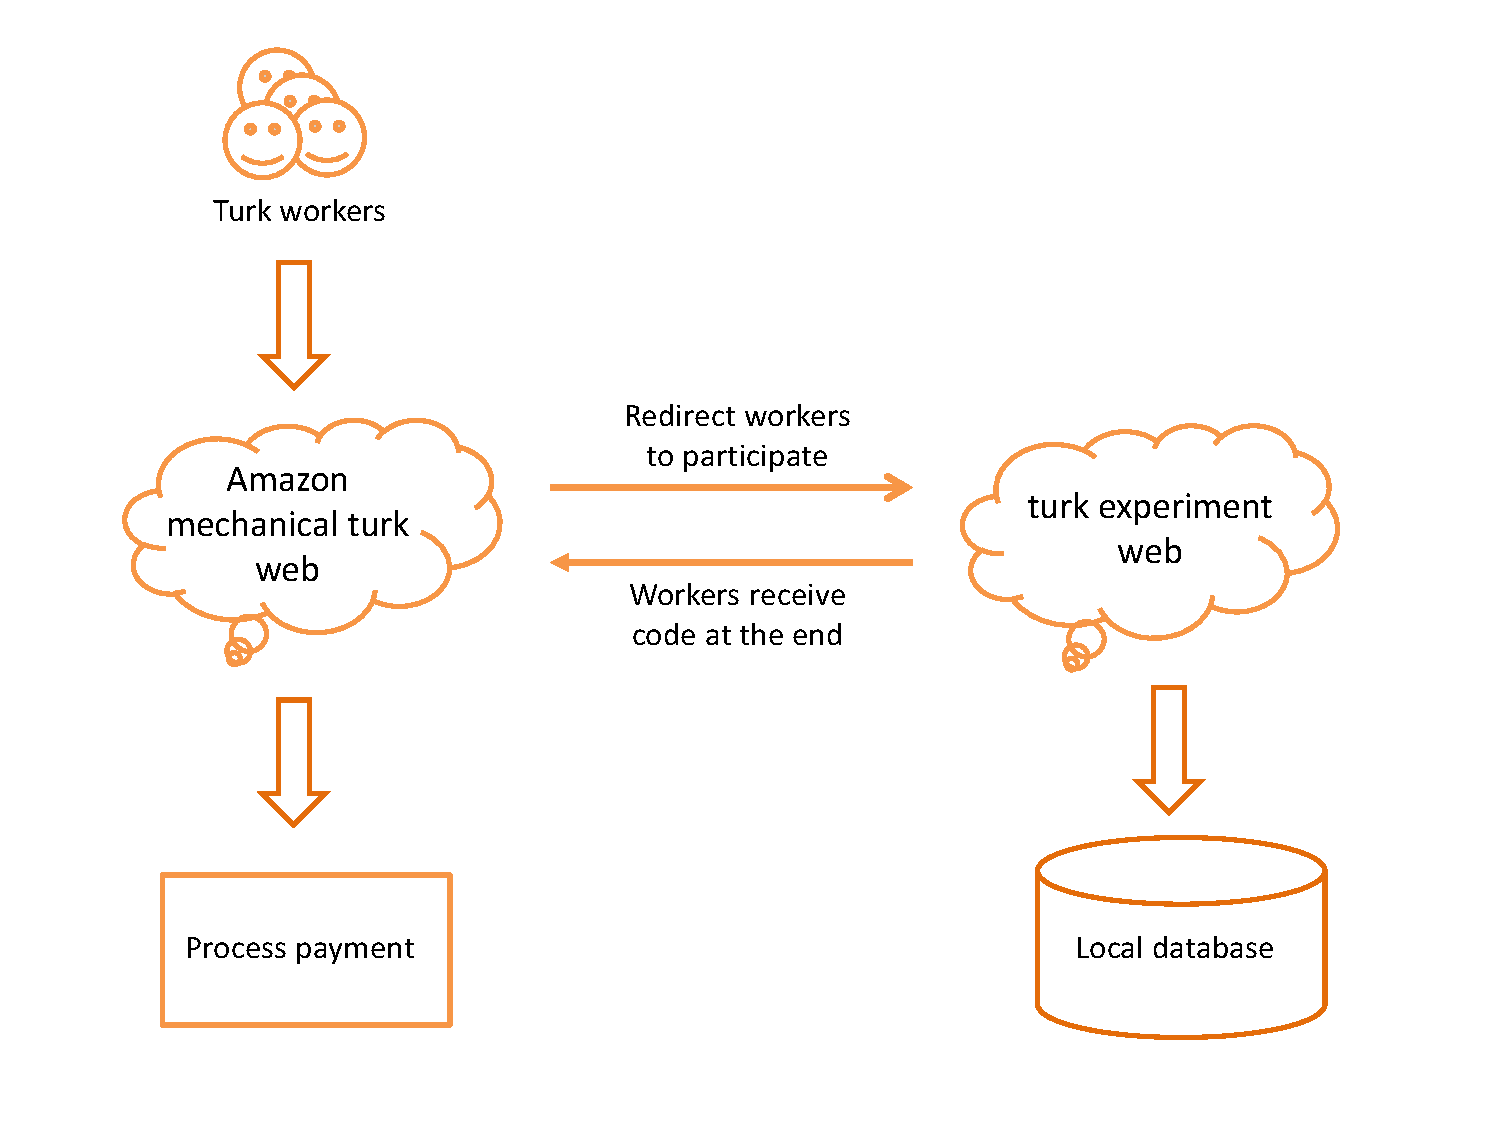
\includegraphics{turk_work_flow.pdf}}
       \caption{Amazon Mechanical Turk workflow and data collection.}
       \label{fig:turk_work_flow}
\end{figure}


\section{Experimental Design} \label{sec:exp_design}

\subsection{Selecting Parameter of Simulation Experiment} The first consideration for a simulation experiment is to fix the parameters of the model of interest. The very first consideration is the sample size. Other parameters depends on the model of interest. For example we have fixed the parameters in our first Amazon Mechanical Turk experiment as shown in table \ref{tbl:experiment_params}.

\subsection{Sample size estimation} For a given proportion $p$ we want to have margin of error (ME) to be 0.1. Thus we have $$ME =1.96 \sqrt{ \frac 1 n p(1-p)} \le 0.05$$ which gives us the estimation of minimum sample size $$n \geq \frac{p(1-p)}{(0.05/1.96)^2}.$$ Now from the theoretical power curve for each parameter combinations shown in table \ref{tbl:experiment_params} we know the power(say $p$) and thus we can estimate the sample size required for that specific combinations of parameter. We collect data such that each of the parameter combinations in the table \ref{tbl:experiment_params} has approximately the estimated sample size that we calculated here.


\subsection{Procedure to simulate plots for survey} \label{sec:simulate_plot} In the simulation study the very first step is to generate a random sample of data from model of interest for prespecified parameters. We call this data set observed data. While the effect of the natural variability of this data set could be contolled by taking the replication of few samples, it is desirable to study whether we can reduce this variability alternatively. The main reason is to minimize the cost. To make sure that the observed data set truly represents model of interest we are considering three approaches. One is Kolomogorov test statistic approach and the other two approaches are quantiles of p values and closeness of estimated parameters to the true parameters. These three approaches are discussed below.\\

{\bf Kolomogorov test statistic approach:} In this approach we simulate 1000 data sets and obtain Kolmogorov test statistic for each set of data as below. $$D_n=\sup_x |F_n(x)-F(x)|$$ where $F_n(x)=\frac1n \sum_{i=1}^n I_{X_i\le x}$ be the empirical distribution function of fitted residuals, $I_{X_i\le x}$ be the indicator function equal to 1 if $X_i\le x$ and equal to 0 otherwise and $F(x)$ be the cumulative function of normal with mean zero(0) and variance $\sigma^2$. We then keep the data set that has minimum value for Kolmogorov test statistic.  For replication purpose we can generate three observed data sets in similar way.\\

{\bf Quantiles of p-value approach:} With any data set we generate there is a p-value associated with testing $H_0: \beta=0$. In this approach we generate 1000 data sets from the model of interest and obtain p-values associated with $H_0: \beta=0$ for each data set after fitting the same model. Then we construct blocks of p-value such as (0.0-$q_{33}$), ($q_{33}$-$q_{66}$), ($q_{66}$-1) where $q_i$ is the $i$th percentile in the distribution of the p-values. We then randomly select three data sets that have corresponding p-values in the above quantile range. As an example the distribution  of p-values in 1000 simulated data sets for $n$=300, $\beta$=3 and $\sigma$=12 is shown in figure \ref{fig:dist_pvalue}.  Notice that if we like to have three replications of plots, we will have observed data sets with smaller p-values as the distribution is highly right skewed as well as the 33th and 66th percentiles of p-values are 0.0101 and 0.077 respectively. So, another option may be to take the mid points of those quantile ranges and pick the data sets that have those p-values.\\

\begin{figure}[hbtp]
   \centering
       \scalebox{.3}{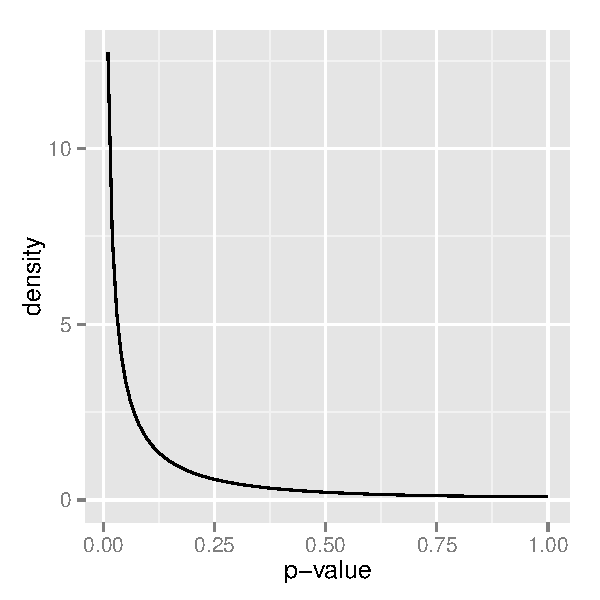
\includegraphics{dist_pvalue.pdf}}
       \caption{Distribution of p-values for $n$=300, $\beta$=3 and $\sigma$=12.}
       \label{fig:dist_pvalue}
\end{figure}

{\bf Closeness of estimated parameters:} When we simulate a data set from the model of interest and again fit the same model with the data set we do not get the parameters estimates same as what we fixed while simulation. It depends on what the standard errors of the parameter estimates are. In our experimental setting we some times have very different estimates for small parameter values(such as one may get estimated value of 0.5 for true $\beta=3$). In this approach we pick the data set that shows most close estimates of parameters compared to true parameter values.\\

All of these three approaches discussed above has some problems. Kolmogorov method does not necessarily make sure that estimated parameters are close to the true parameters. On the other hand closeness of estimated parameters does not make sure that p value is small enough when we should reject the null hypothesis. Only the quantiles approach seems reasonable as it has much control over p-values and it gives similar data sets that has closest parameter estimates. So we used the quantiles of p-value approach in section \ref{sec:simulate_plot} to obtain three replicated sample of observed data sets for a particular parameter settings.\\

\section{Website to Run the Turk Experiment} We developed a web site to run the Amazon Mechanical Turk experiments.  PHP scripting language is used and embedded with HTML for designing the web site. Javascript is used for validating the input data and producing warning message.  We use  Amazon Mechanical Turk web site to recruit the participants and direct them to our web site to actually participate in the survey. This has allowed us to get the data directly in a secure way from the web and we don't have to depend on the Mechanical Turk web site to transfer data to our server. 

\subsection{Data collection} To collect the survey data we developed a web site that shows a plot to an individual and get feedback from that individual. Each individual is asked to provide feedback for at least 10 different plots. The 10 plots that are shown to an individual are randomly chosen with probability proportional to the number of responses required (the sample size) for that plot.

The information collected from each individual is shown in table \ref{tbl:data_info}. Data received from each individual are automatically saved in a secured mysql server maintained by the department of statistics, Iowa state university. 

\begin{table}[hbtp]
\caption{Information Collected from Each Individual}
\centering 
\begin{tabular}{lp{8cm}} 
\hline
Information &  Description \\ %[0.5ex] % inserts table %heading 
\hline
Identification & Nick name or any ID to determine the responses of an Individual \\
Response number & The number of the plot on the lineup plot which the individual thinks the most different than other 19 plots.\\ 
Reason of of choice & Reason why the individual chooses the plot \\
Confidence level & Confidence level of individual choice \\ 
Age group& The age group where the individual belongs \\
Education & The highest level of education completed \\
Gender & Male or female \\
Geographic Location & This information is collected through the ip address of the individual computer \\ 
Time taken & Time taken for each feed back\\
\hline
\end{tabular}
\label{tbl:data_info}
\end{table}	


\subsection{Data collection sequence} Once turk users are directed to our web site, they can see the detailed explanation on how they can perform the task of evaluation. Some simple examples are displayed along with correct responses. The users have options to try some test lineups before going for the actual experiment. But before that they have to provide the informed consent as per IRB requirement. The flow chart for this is shown in Figure \ref{fig:turk_data_flow}

\begin{figure}[hbtp]
   \centering
       \scalebox{.4}{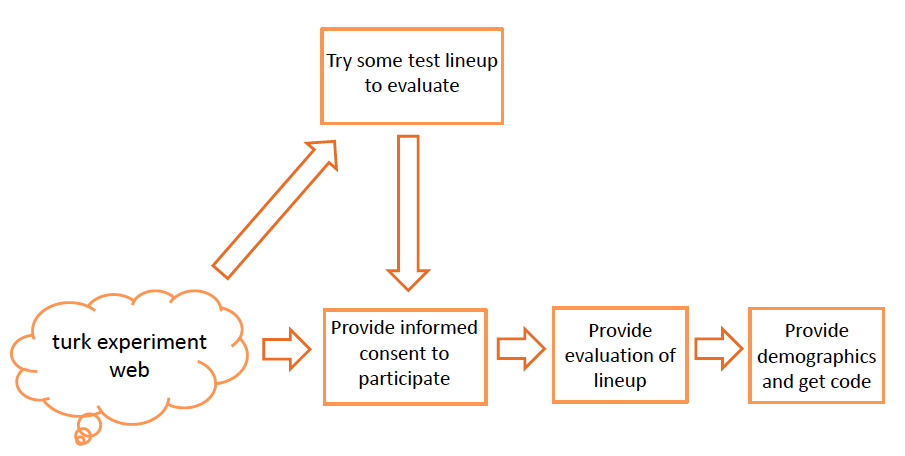
\includegraphics{turk_data_flow.png}}
       \caption{Data collection work flow. Turk worker can try some test lineups before going to the live experiment after providing informed consent.}
       \label{fig:turk_data_flow}
\end{figure}

Two web forms are designed to collect information from the turk users. The first form shown in Figure \ref{fig:turk_web} collects feedback information about a single lineup. The information collected through this form is all about the lineup that includes plot number selected, reasons for selection and the confidence level of the selection. Each turk user is identified by the nick name which is mainly the turk ID. 

Each turk user is shown some specific number of lineups for evaluation. These lineups are randomly selected from a pool of lineups designed for evaluations. The algorithm for how the lineups should be selected to show and what would be the order of display is implemented in the form shown in Figure \ref{fig:turk_web}. Also there is a check for invalid information which is implemented using javascript. If users try to go forward without giving any feedback they are not allowed to do that showing a warning message.

\begin{figure}[hbtp]
   \centering
       \scalebox{.4}{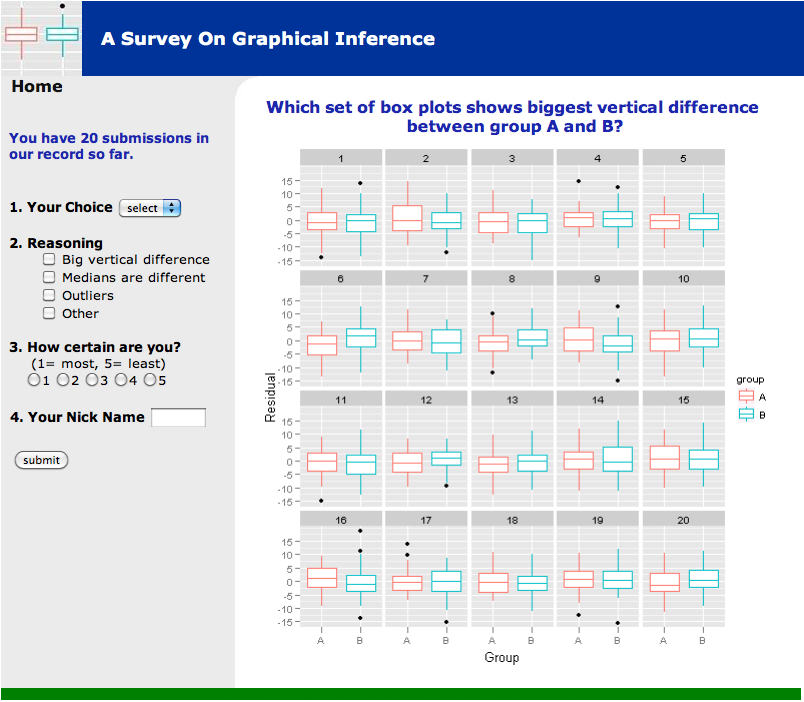
\includegraphics{turk_web.png}}
       \caption{A sample data collection form. Lineups are presented at random for evaluations by the turk workers.}
       \label{fig:turk_web}
\end{figure}

After the evaluation is recorded on a lineup through form shown in Figure \ref{fig:turk_web} another form shown in Figure \ref{fig:turk_web_feedback} is used to give feedback to the turk users whether they correctly identifies the true plot and how many evaluations are recorded from the users. This form is also used to collect demographic and educational information about the user. After the required number of evaluations are obtained from each turk user, a pass code is given as a proof of the completion of the task which then later used for payment purpose.

\begin{figure}[hbtp]
   \centering
       \scalebox{.4}{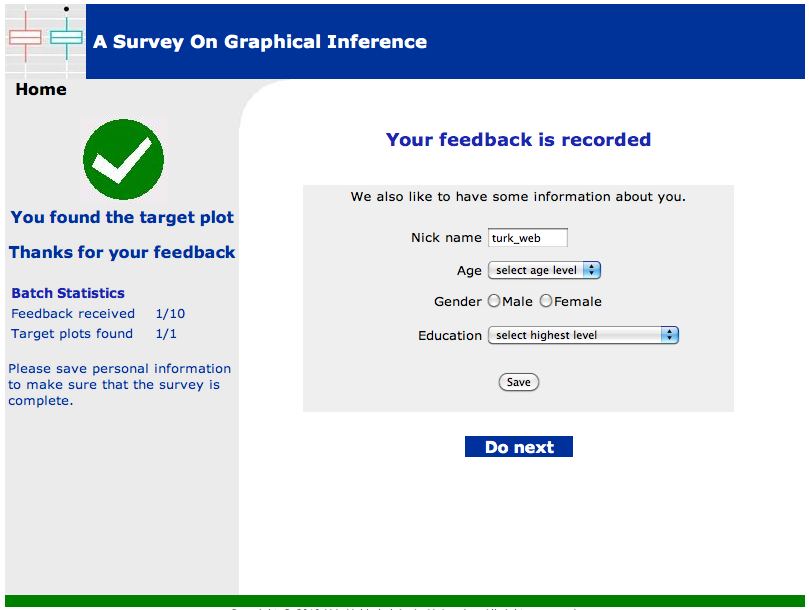
\includegraphics{turk_web_feedback.png}}
       \caption{The turk workers are given feedbacks whether their evaluation for each lineup was correct or not. This works as an incentive for the worker to work more enthusiastically. To ensure the payment, the turk workers have to provide some information using this form.}
       \label{fig:turk_web_feedback}
\end{figure}

\subsection{Database design} The design of the database to store the collected data is shown in Figure \ref{fig:turk_database_design}. It is designed such a way that data from many different experiments can be stored in the same database. In total five separate tables are used. Table turk\_worker contains static information about each turk worker. The location information of each turk worker is stored in ip\_detals table. The information in this table is collected later based on the ip address of each turk worker. Table picture\_delais contains the static information about each lineup. Table feedback is a dynamic table that grows with the number of feedbacks from each turk user. The multiple activities of each turk user are recorded in turk\_activity table. This table also contains the codes provided to the user once they finish the experiment. For our web site we used MySQL database located on a local server.

\begin{figure}[hbtp]
   \centering
       \scalebox{.4}{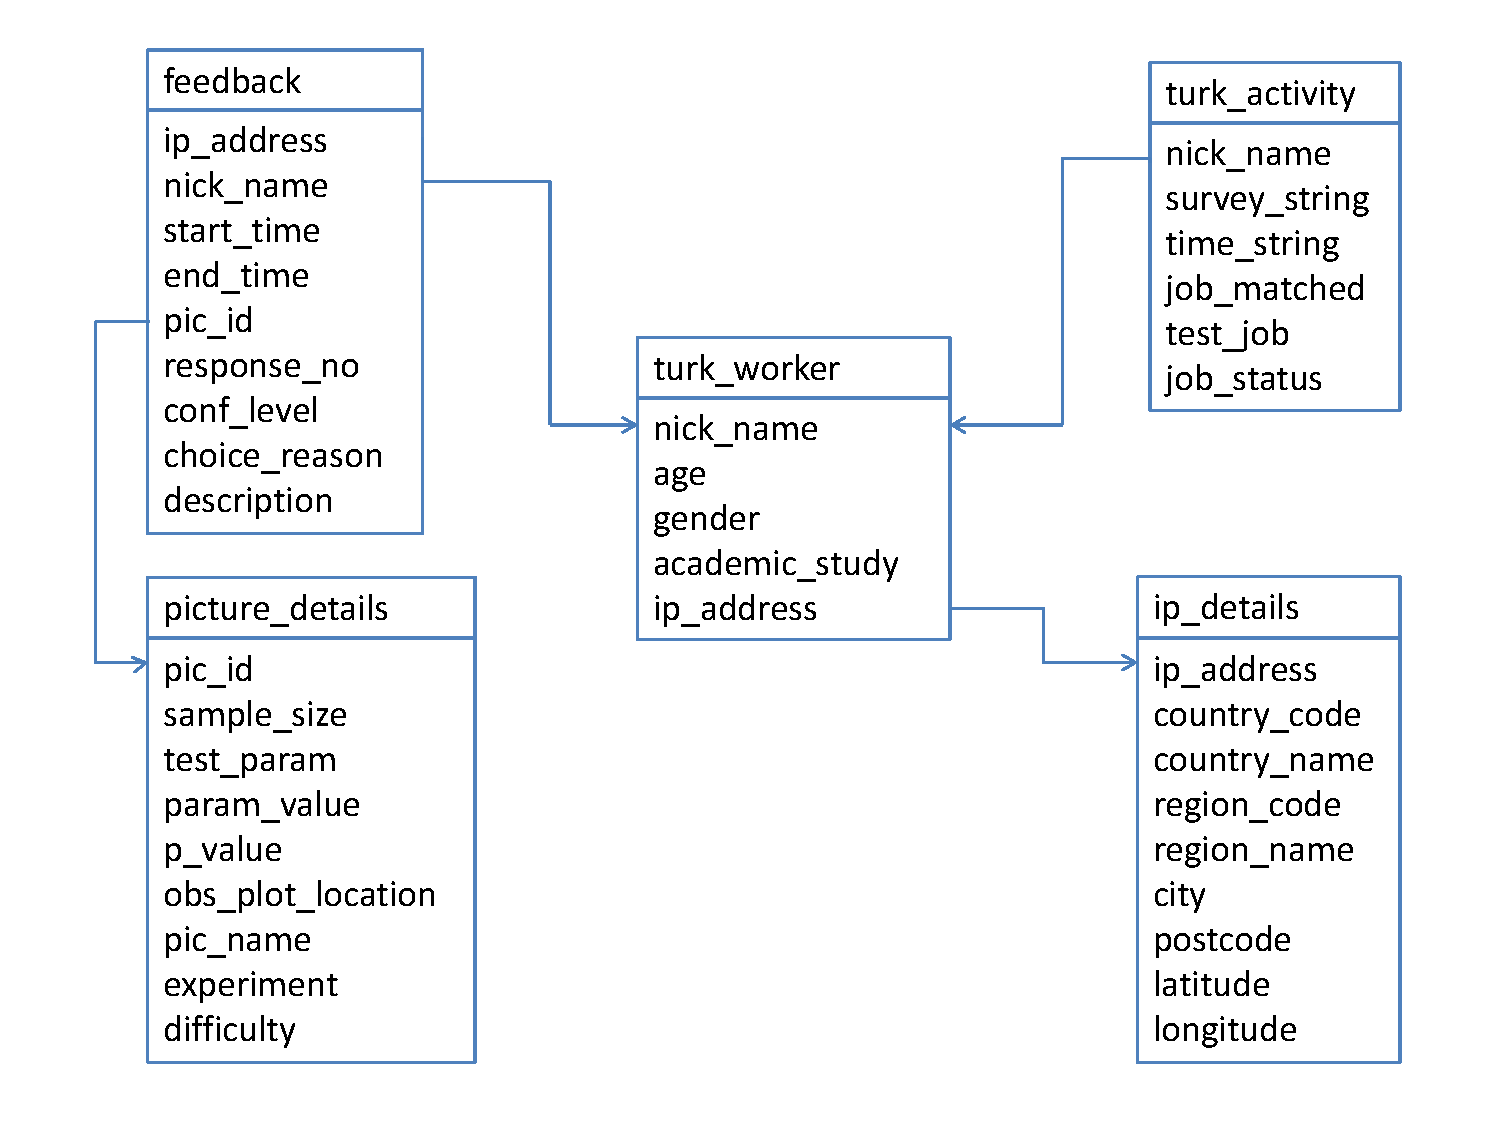
\includegraphics{turk_database_design.pdf}}
       \caption{Database design for Turk experiment data collection. The same database can be used for multiple turk experiments by keeping experiment information in picture details table which contains information about the lineups.}
       \label{fig:turk_database_design}
\end{figure}

\section{Payment of Turk Worker} Turk workers are usually small payee workers. There several issues related to the payment of their effort. These are briefly discussed in the following section and we intend to work more on this as we progress through this dissertation work. 


\begin{table}[hbtp]
\caption{Number of task submitted by the turk workers, number of task got rejected and total task completion time for each of the different experiment indicate the performance of turk workers. Majority of the tasks are rejected for boxplot experiment and the payment per task was the lowest for this experiment.}
\centering 
\begin{tabular}{clccccc} 
\hline
Experiment &  Plot & Submitted & Rejected & Duration & Pay/Task \\ %[0.5ex] % inserts table %heading 
\hline
1 & Boxplot & 406 & 106 & 527340 & 0.5\\
2 & Scatterplot & 359 & 9 & 153660 & 1\\
3 & Contaminated plot & 219 & 19 & 454200 & 1\\
4 & Polar vs Cartesian & 110 & 10 & 41940 &1\\
5 & Hist vs density & 234 & 37 & 149640 & 1\\
6 & Violine vs boxplot & 417 & 17 & 381120 &1 \\
7 & Group separation & 106 & 6 & 18540 &1\\
8 & Sine Illusion & 101 & 1 & 282180 &1\\
\hline
\end{tabular}
\label{tbl:worker_performance}
\end{table}	

\begin{figure}[hbtp]
   \centering
       \scalebox{.6}{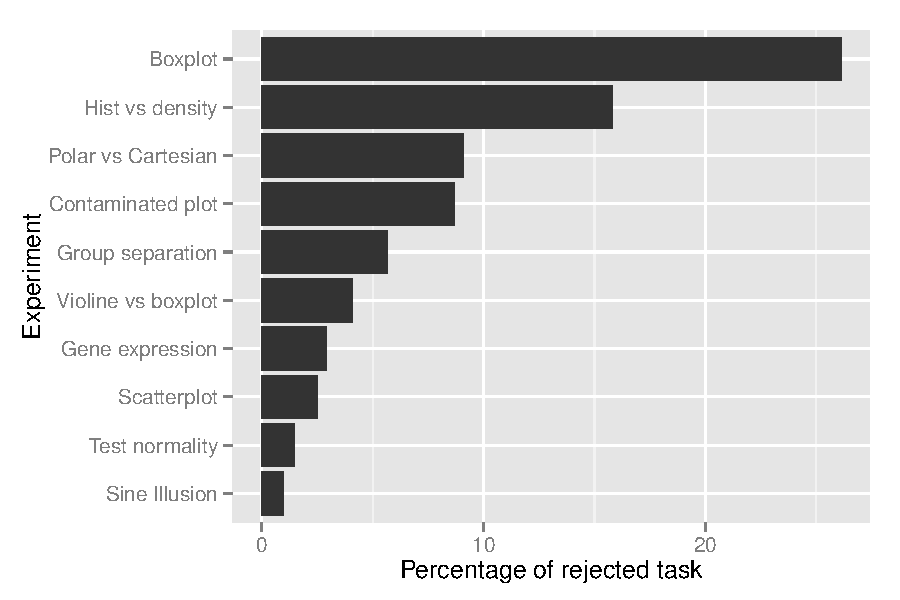
\includegraphics{rejected_task.pdf}}
       \caption{Percentage of rejected task for various experimental plot type.}
       \label{fig:rejected_task}
\end{figure}

\subsection{Wage Rate for the Turkers}Amazon Mechanical Turk suggest that each worker gets \$6/hour as wage. Thus we need to estimate how much time a tusk may take to complete and based on that we have to specify the payment for each task. Our experience indicates that a better payment lures more serious workers who usually provide cleaner data which is more reliable. We may study this issue while we do multiple turk experiments.

\subsection{Accepting or Rejecting Payments for Turk Evaluation} In our design we keep a test lineup plot which is very easy to evaluate. The general criteria may be to reject payment when workers do not get that easy test lineup plot. Our experience suggest that there are workers who did not get that test plot but their overall success rate is very high. So depending on only one criteria the payment should not be made. These issues would be addressed in our future work based on the several turk experiments that we intend to carry out.


\section{What do people pick, $R^2$ or p-value?} What do people pick in a lineup plot, p-value or $R^2$? To address this issue we obtain the approximate theoretical relationship between $R^2$ and the power of the classical hypothesis test. Suppose we want to test the significance of the slope ( i.e.,  $H_0: \beta=0$ against $\beta \ne 0$) of a continuous covariate $X$ in  a simple linear regression model setting. Also consider $X \sim N(0,1)$. For a sample of size $n$ this gives us 
\begin{eqnarray*}
Y_i-\bar{Y}& = & \beta_0+\beta_1X_i+\epsilon_i - \beta_0 - \beta_1 \bar{X}- \bar{\epsilon} \\
          & = & \beta_1(X_i-\bar{X})+(\epsilon_i-\bar{\epsilon})
\end{eqnarray*}
Now 
\begin{eqnarray*}
X_i-\bar{X}& = & X_i - \frac1n (X_1 + X_2 + ... + X_i + .....+ X_n) \\
          & = & X_i - \frac1n X_i - \frac1n \sum_{j \neq i}{X_j}\\
          & = & (1-\frac1n)X_i - \frac1n \sum_{j \neq i}{X_j}
\end{eqnarray*}

Thus we have 
\begin{eqnarray*}
E(X_i-\bar{X})^2 & = & (1-\frac1n)EX_i^2 - \left( \frac1n \right )^2 (n-1) EX_j^2 \\
                 & = & (1-\frac1n)^2+ \frac{n-1}{n^2}\\
                 & = & \frac{n-1}{n}
\end{eqnarray*}

Similarly we have 

\begin{eqnarray*}
E(\epsilon_i-\bar{\epsilon})^2 & = & (1-\frac1n)E\epsilon_i^2 - \left( \frac1n \right )^2 (n-1) E\epsilon_j^2 \\
                 & = & \left((1-\frac1n)^2+ \frac{n-1}{n^2} \right) \sigma^2 \\
                 & = & \frac{n-1}{n}\sigma^2
\end{eqnarray*}
Finally we have expected total sum of square (SST) as
\begin{eqnarray*}
E\sum_i{(Y_i-\bar{Y})^2} & = & \sum_i E(Y_i-\bar{Y})^2=\sum_i \left [ \beta_1^2 E(X_i-\bar{X})^2 + E(\epsilon_i-\bar{\epsilon})^2 \right] \\
                 & = & \sum_i\left[ \beta_1^2 \frac{n-1}{n}+  \sigma^2 \frac{n-1}{n}\right]\\
                 & = & (n-1)(\sigma^2+\beta_1^2)
\end{eqnarray*}

We know $E(MSE|X) = \sigma^2$ or $E(SSE/n-2)|X = \sigma^2$ which gives the expected residual or error sum of square as $$E \sum_i (Y_i-\hat Y_i)^2=(n-2)\sigma^2$$
Thus we have the expected regression sum of squares $SSR =  (n-1)(\sigma^2+\beta_1^2) - (n-2)\sigma^2 = (n-1) \beta_1^2+\sigma^2$ This gives $$R^2=\frac{(n-1) \beta_1^2+\sigma^2}{ (n-1)(\sigma^2+\beta_1^2)}$$


\begin{figure}[hbtp]
   \centering
       \scalebox{.3}{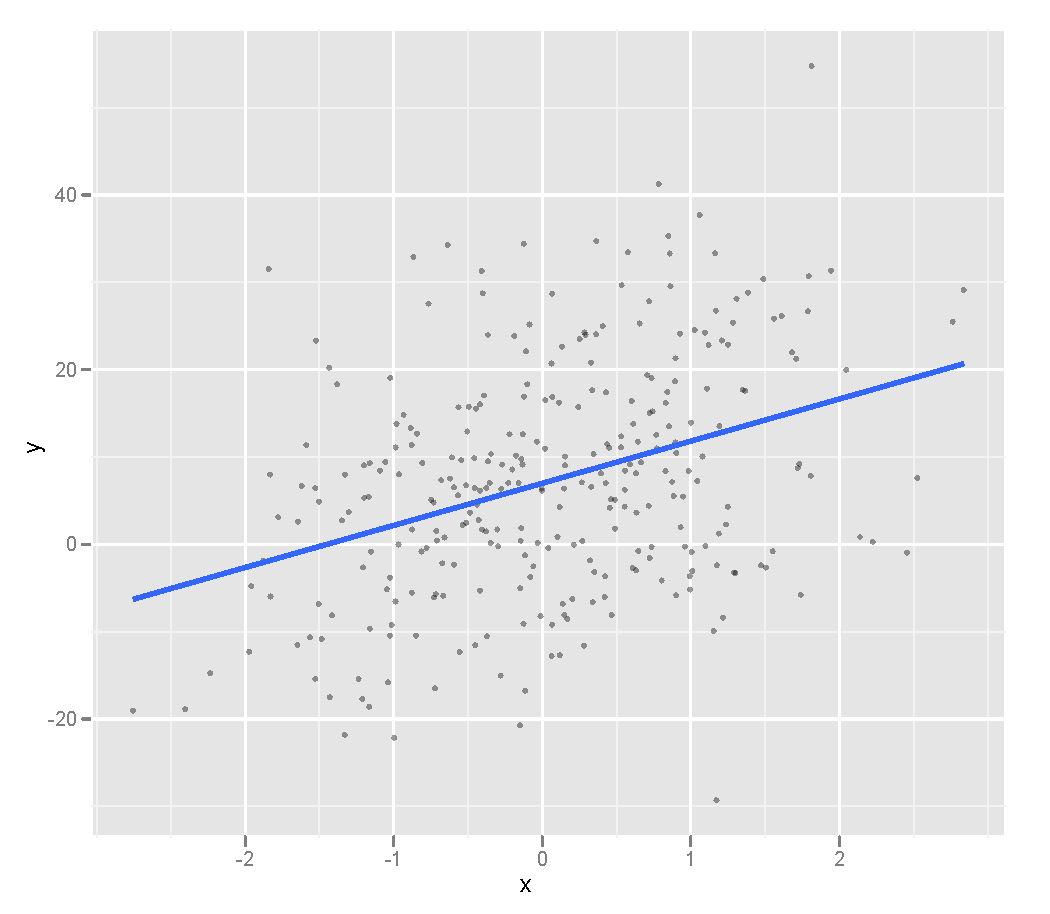
\includegraphics{scatter_plot_beta_4.pdf}}
       \caption{Scatter plot of data generated for $\beta_0$=6, $\beta_1$=4, sample size $n =300$ and $\sigma = 12$. $R^2$ for this data was obtained as 0.1309 showing that the model could not successfully explain the variation in $Y$. But notice in figure \ref{fig:power_rsq} that power for $\beta$=4 is almost 1. So, Can we conclude that $R^2$ does not have any effect in deciding whether $H_0: \beta_1=0$ should be rejected or not?}
       \label{fig:plot_beta_4}
\end{figure}


\begin{figure}[hbtp]
   \centering
       \scalebox{.35}{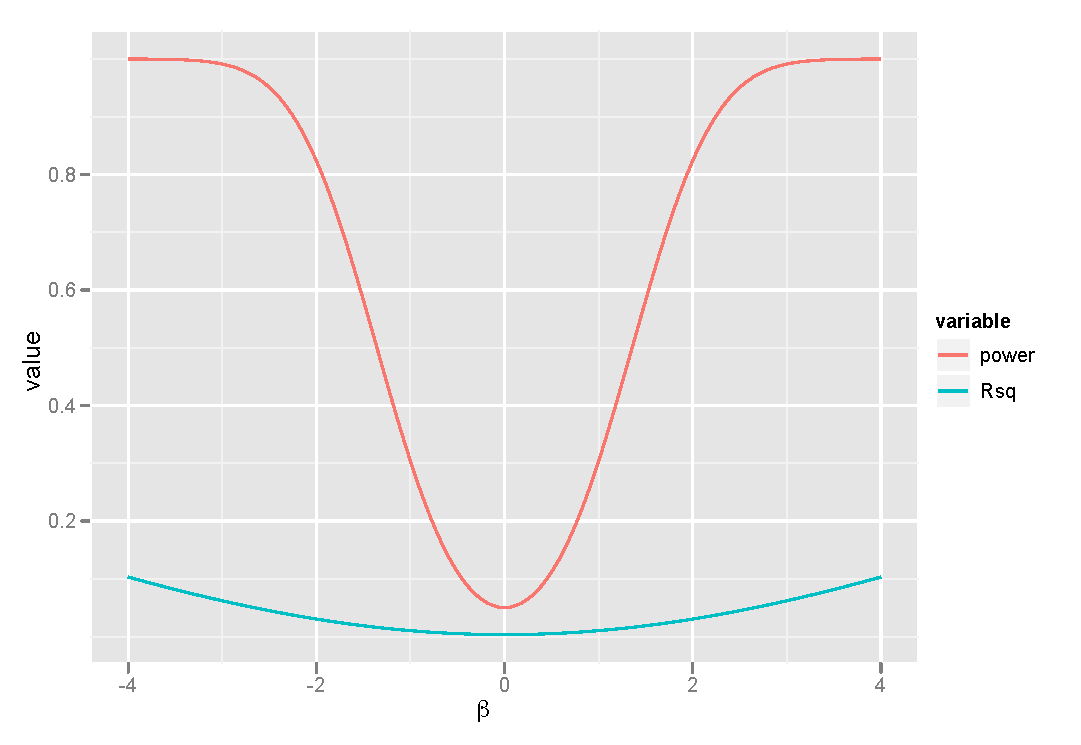
\includegraphics{power_300_12.pdf}}
       \caption{Power curve and $R^2$ values for sample size $n =300$ and $\sigma = 12$. Notice that for a small value of $R^2$ (0.1) the power is almost 1.}
       \label{fig:power_rsq}
\end{figure}


\begin{figure}[hbtp]
   \centering
       \scalebox{.35}{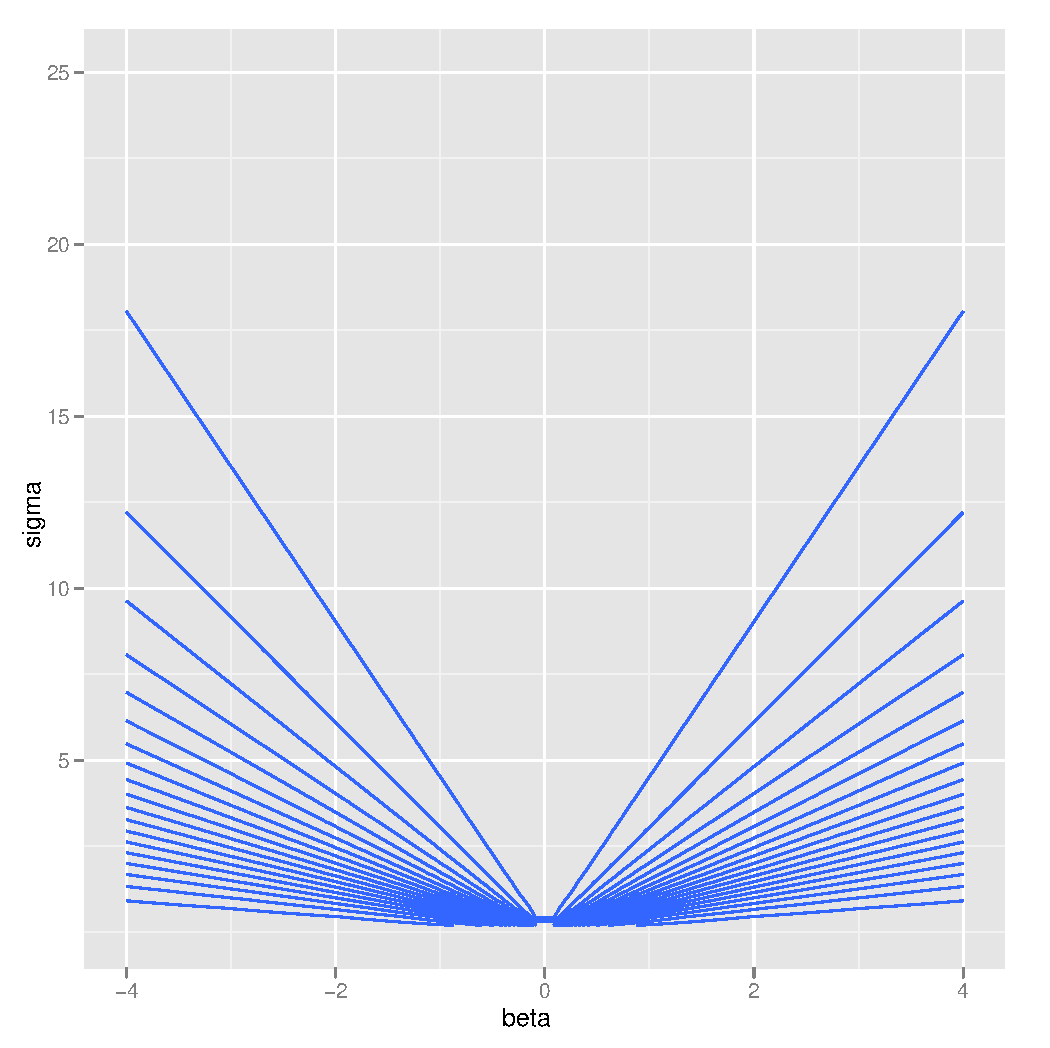
\includegraphics{rsquare_contour.pdf}}
       \scalebox{.35}{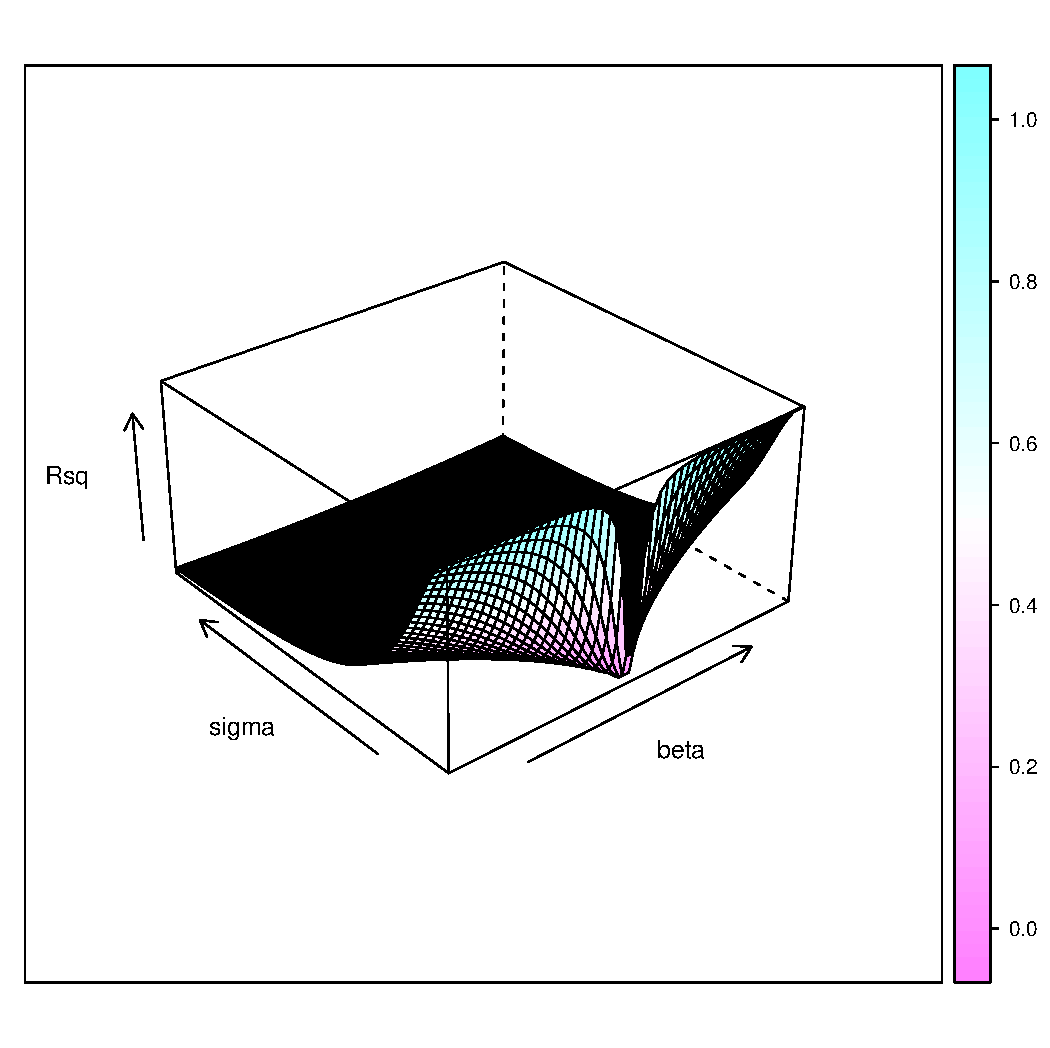
\includegraphics{rsquare_beta_sigma.pdf}}
       \caption{Contour and surface plots of $R^2$ for sample size $n =300$. The values for $R^2$ goes down sharply with $\sigma$ and $\beta$.}
       \label{fig:contour_rsq}
\end{figure}

\begin{figure}[hbtp]
   \centering
       \scalebox{.35}{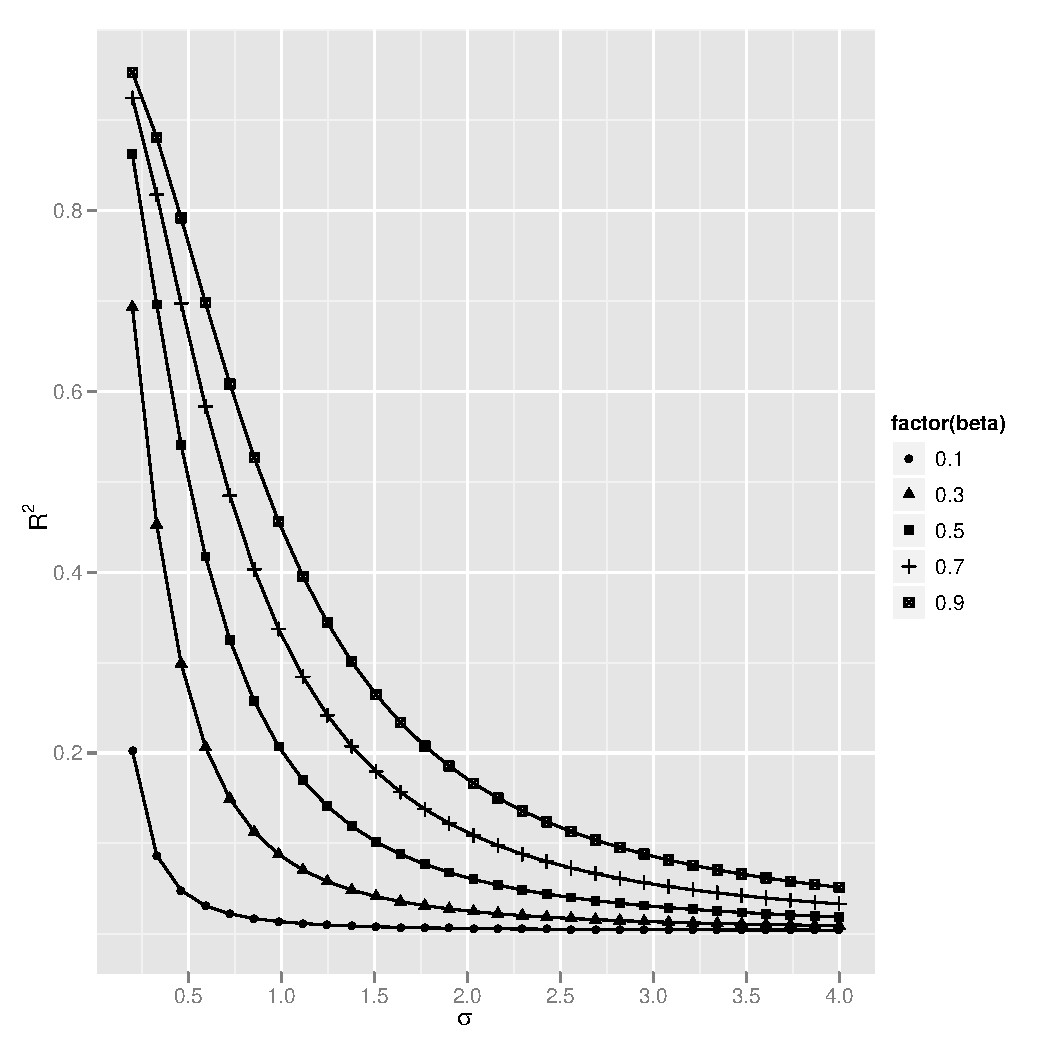
\includegraphics{rsquare_beta_sigma_lines.pdf}}
       \scalebox{.35}{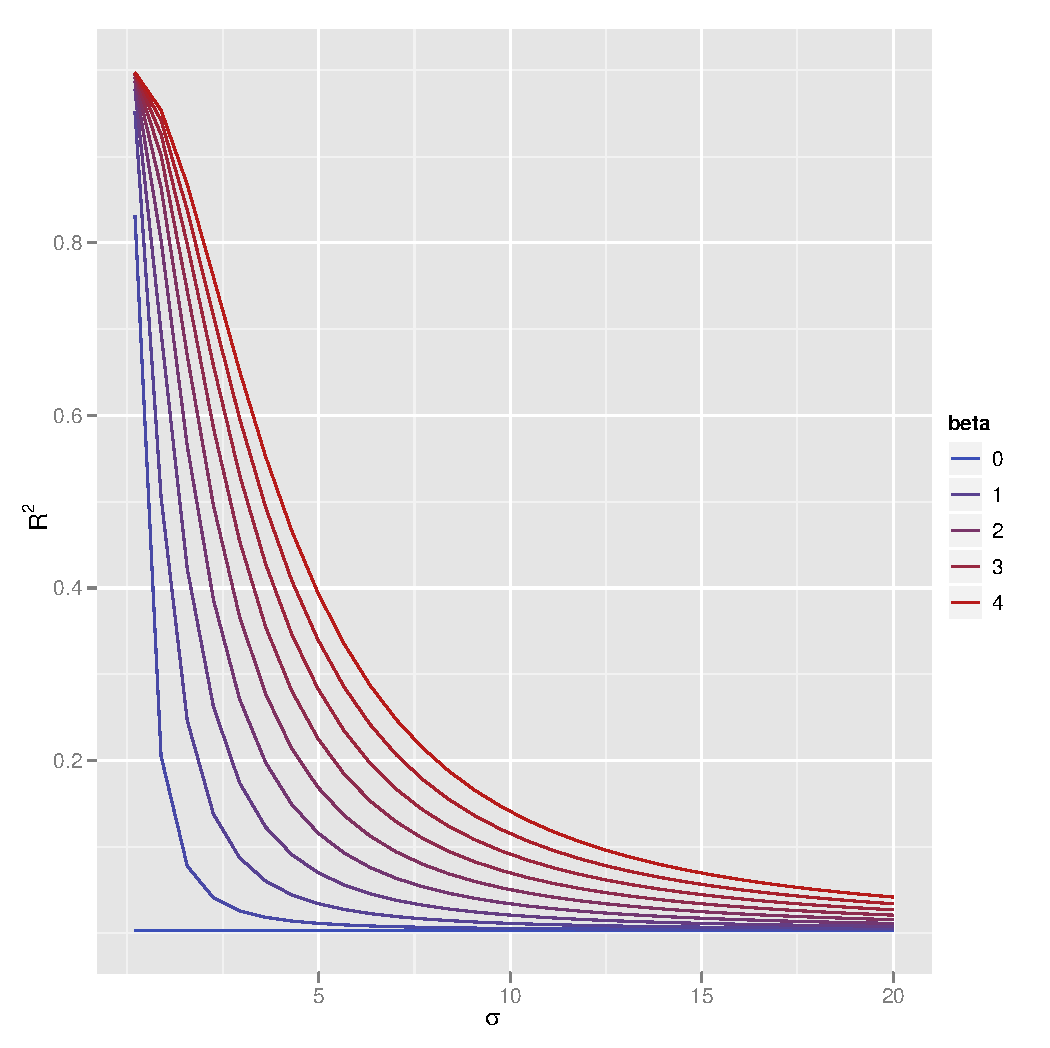
\includegraphics{rsquare_beta_sigma_lines1.pdf}}       
       \caption{Relationship of $R^2$ with $\sigma$ and $\beta$ for sample size $n =300$. The values for $R^2$ goes down sharply with $\sigma$ and $\beta$.}
       \label{fig:rsq}
\end{figure}


\section{Performance} In this section we intend to analyze the performance of the experiments we did using Amazon Mechanical turk. We have feed back data for the similar plots from both turk workers as well as from the people who regularly participates in the graphics group meeting of our department. We consider later participants as more knowledgeable and trained in seeing pattern in statistical plots. We can use these data to evaluate the performance of the general participants from around the world.

\section{Quality of Turk Data}

\subsection{Data Cleaning}

\subsection{Diversity in the Data}

\begin{figure}[hbtp]
   \centering
       \scalebox{.5}{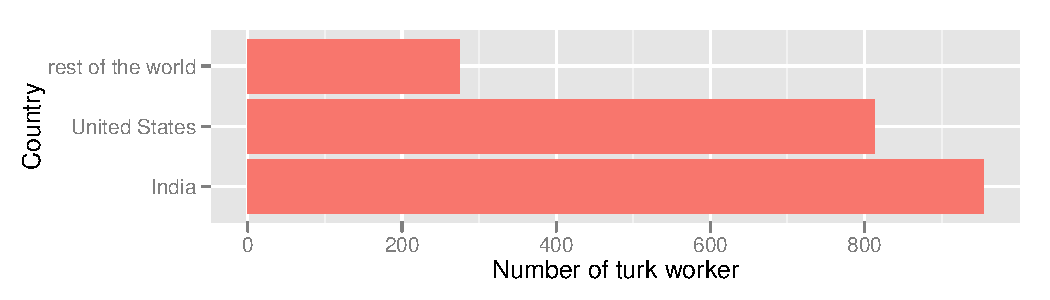
\includegraphics{turker_country.pdf}}
       \scalebox{.5}{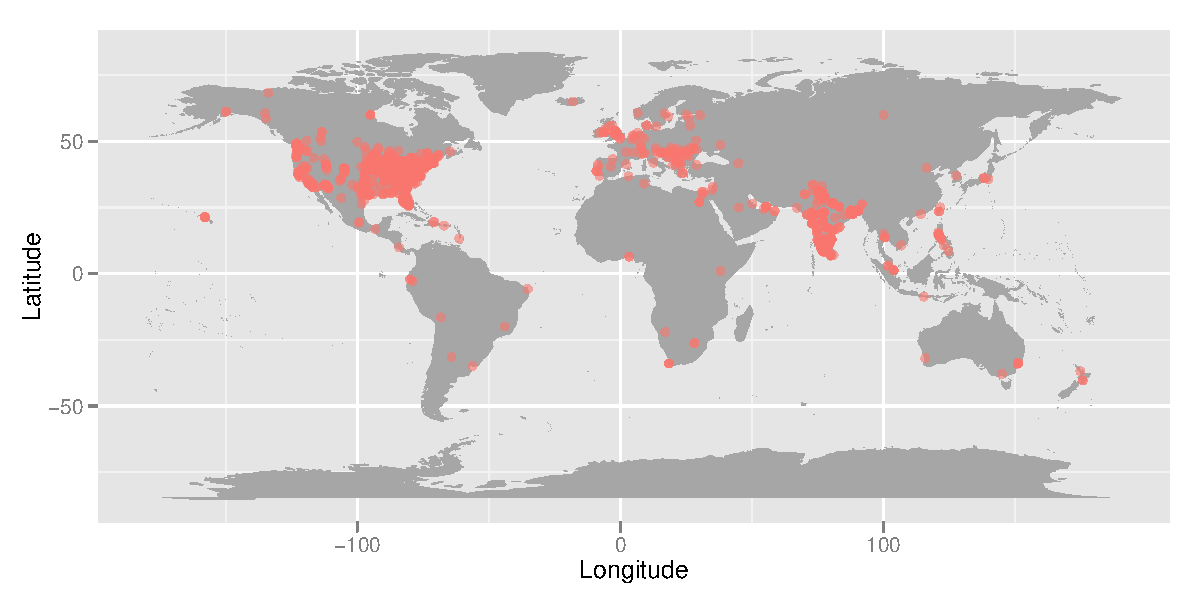
\includegraphics{turker_location.pdf}}       
       \caption{The location of turk workers on the world map shows the geographical diversity of turk workers even though most of the workers come from India and United States.}
       \label{fig:rsq}
\end{figure}

\subsection{Selection Bias} Since data are collected through web interface it is possible to have the selection bias in the turk experiment we did. In this section we intend to analyze to what extent this selection bias has occurred and how we can adjust for this.


\section{Conclusion}

\bibliographystyle{plain}
\bibliography{references} 

\end{document}





























































\documentclass{article}
\usepackage{times}
\usepackage{natbib}
%\usepackage{multicol}
%\RequirePackage{natbib}
\usepackage{amsmath, amssymb, fullpage, amsthm, array, algorithm2e,graphicx}
%\usepackage[dvips]{graphics}

\graphicspath{{images/}}
\usepackage{color}
\newcommand{\blue}[1]{{\color{blue} #1}}
\newcommand{\red}[1]{{\color{red} #1}}

\setlength{\oddsidemargin}{0in}
\setlength{\evensidemargin}{0in}
\setlength{\textwidth}{6.5in}
\setlength{\topmargin}{-0.4in}
\setlength{\textheight}{9in}
\evensidemargin \oddsidemargin

\newtheorem{thm}{Theorem}[section]
\newtheorem{dfn}{Definition}[section]
\newtheorem{cor}{Corollary}[thm]
\newtheorem{con}{Conjecture}[thm]
%\setlength{\parindent}{0in}   % for no indent

%\topmargin -0.10in   % when making pdf
%\textheight 9.15in  % when making pdf

\setlength\parindent{0pt}



% Article top matter
\title{Turk Experiments for Visual Inference}
\author{Mahbubul Majumder, Heike Hofmann, Dianne Cook\\
        Department of Statistics, Iowa State University}
%\date{\today}  %\today is replaced with the current date


\begin{document}


\maketitle



\begin {abstract} 

It has been found that the visual test, which does not have
distributional assumptions, has the power comparable to the classical
tests [3]. To examine the power of visual statistical inference we
recruited human subjects from Amazon Mechanical Turk \cite{turk}  for
evaluating lineups[1,2]. The Turk website is designed to recruit
workers for simple and easy tasks. Even though the task of evaluating
lineups is easy, the technical design of the experiment is complex and
the tools available to design this from Turk website is just too
simple. In this paper we present how we deal with this trouble and to
conduct our experiment.



Statistical graphics play a crucial role in exploratory data analysis, model checking and diagnosis. Until recently there were no formal visual methods in place for determining statistical significance of findings. This changed, when \citet{buja:2009} conceptually introduced two protocols for formal tests of visual findings. In this paper we take this a step further by comparing the lineup protocol \citep{buja:2009} against classical statistical testing  of the significance of regression model parameters. A human subjects experiment is conducted using simulated data to provide controlled conditions. Results suggest that the lineup protocol provides results equivalent to the uniformly most powerful (UMP) test and for some scenarios yields better power than the UMP test.
\end {abstract}



%\begin{multicols}{2}
%\twocolumn

\section{Introduction} 

Any statistical analysis must include some statistical graphics. For exploratory data analysis, statistical graphics play an invaluable role in model checking and diagnostics. Even though we have established mathematical procedures to obtain various statistics, we need to support the results by also producing the relevant plots. 


\bibliographystyle{plain}
%\bibliographystyle{asa}
\bibliography{references}

\end{documents}

Any statistical analysis must include some statistical graphics. For exploratory data analysis, statistical graphics play an invaluable role in model checking and diagnostics. Even though we have established mathematical procedures to obtain various statistics, we need to support the results by also producing the relevant plots. 

The scientific foundation of graphical methods for data analysis is well established by \cite{cleveland:1984}. In recent years we have seen several major advances in statistical graphics. Modern computing systems like R and SAS ease the production of high quality statistical plots. A grammar of graphics introduced by \cite{wilkinson:1999} presents a structured way to generate specific graphics from data and define connections between disparate types of plots.  \cite{hadley:2009} has implemented a revised version of the grammar of graphics in R, in the package {\tt ggplot2}.   \blue {Graham Wills has implemented the grammar in SPSS, but I'm not sure how to cite this.}


\citet{buja:2009}, following from \cite{gelman:2004}, proposed two protocols that allow the testing of discoveries made from statistical graphics. This work represents a major advance for graphics, because it bridges the gulf between classical statistical inference procedures and exploratory data analysis.

In this paper we compare graphical inference to classical statistical inference for a set of regression type example. We also present results of a human-subject study assessing the performance of individuals on lineup plots \citep{buja:2009} for testing significance of regression parameters. 

Section \ref{sec:visual_test} describes the basic ideas of visual inference, Section \ref{sec:regression} applies these ideas to the case of inference for regression analysis. In Section \ref{sec:simulation} we outline the setup for the human-subject study and  and present results. 


\begin{table*}[hbtp]
\caption{Comparison of visual inference with existing inference technique}
\centering 
\begin{tabular}{llll} 
\hline
  & Mathematical Inference &  Visual Inference \\ %[0.5ex] % inserts table %heading 
\hline
  Hypothesis & $H_0: \beta=0$ vs $H_1: \beta \ne 0$& $H_0: \beta=0$ vs $H_1: \beta \ne 0$\\
 & \begin{minipage}[h]{2.5cm} \begin{center} \scalebox{0.2}{\includegraphics{down_arrow.pdf}} \end{center} \end{minipage} & \begin{minipage}[h]{2.5cm} \begin{center} \scalebox{0.2}{\includegraphics{down_arrow.pdf}} \end{center} \end{minipage} \\
				  
 Test statistic & $T(y)=\frac{\hat{\beta}}{se(\hat{\beta})}$ & $T(y)=$ \begin{minipage}[h]{1cm} \begin{center} \scalebox{0.45}{\includegraphics{stat_category.pdf}} \end{center} \end{minipage} \\
				 
 & \begin{minipage}[h]{2.5cm} \begin{center} \scalebox{0.2}{\includegraphics{down_arrow.pdf}} \end{center} \end{minipage} & \begin{minipage}[h]{2.5cm} \begin{center} \scalebox{0.2}{\includegraphics{down_arrow.pdf}} \end{center} \end{minipage} \\
				 
 Null Distribution & $f_{T(y)}(t); $\begin{minipage}[h]{2.5cm} \begin{center} \scalebox{0.55}{\includegraphics{stat_mathematical_test.pdf}} \end{center} \end{minipage} & $f_{T(y)}(t); $ \begin{minipage}[h]{2.5cm} \begin{center} \scalebox{0.19}{\includegraphics{test_category.pdf}} \end{center} \end{minipage} \\
 & \begin{minipage}[h]{2.5cm} \begin{center} \scalebox{0.2}{\includegraphics{down_arrow.pdf}} \end{center} \end{minipage} & \begin{minipage}[h]{2.5cm} \begin{center} \scalebox{0.2}{\includegraphics{down_arrow.pdf}} \end{center} \end{minipage} \\
 Reject $H_0$ if & observed $T$ is extreme & observed plot is identifiable \\
\hline 
\end{tabular}
\label{tbl:compare}
\end{table*}	

\section{Visual Statistical Inference} \label{sec:visual_test} 
Visual tests are non-parametric tests of the form $H_0$: the data plot is visually not distinguishable from a null plot vs $H_1$: the data plot is visually distinguishable from a plot generated consistently with $H_0$.

Power of a plot and $p$-value have been derived in Buja and Wickham as ...



for this paper, we want to place the parametric inference of a regression setting into the framework of visual testing:



This section outlines the concepts of visual inference in comparison to the procedures of classical statistical inference. Table \ref{tbl:compare} (derived from \citet{buja:2009}) gives a summarized overview of this comparison.

Let $\theta$ be a population parameter of interest, with $\theta \in \Theta$, the parameter space. 
Any null hypothesis $H_0$ then partitions the parameter space into $\Theta_0$ and $\Theta_0^c$, with $H_0: \theta \in \Theta_0$ versus $H_1: \theta \in \Theta_0^c$. 

\blue{Similarly, for any test, we have a rejection region $R$ and, complementary to that, $R^c$,  that partition the space of the test statistic, which is usually a subspace of the real numbers.}
%\subsection{Visual Statistic} 

For visual inference, the statistic is -- unlike in the classical hypothesis test -- not a single value, but a graphical representation of the data chosen to display the strength of the parameter of interest, $\theta$. When the alternative hypothesis is true, it is expected that the plot of the observed data, the test statistic, will have visible feature(s) consistent with $\theta \in \Theta_0^c$, and that visual artifacts will not distinguish the test statistic as different when $H_1$ is not true. We will call a plot with this property a {\it visual statistic} for $\theta$. More formally, 

\blue{

\begin{dfn} \label{dfn:test}
A \textit{visual test (statistic)} $T_\theta$ is defined as the grammar \citep{wilkinson:1999} of the plot,  consisting of type and specification of aesthetics necessary for complete reproducibility.
\end{dfn}
}

\begin{dfn}\label{dfn:lplot}
A lineup plot is a layout of $m$ visual statistics, consisting of 
\begin{itemize}\itemsep-3pt
\item $m-1$ plots simulated from the model specified by $H_0$  (null plots) and 
\item the test statistic produced by plotting the observed data, possibly arising from $H_1$.
\end{itemize}
\end{dfn}

The $(m-1)$ null plots can be considered to be samples drawn from the sampling distribution of the test statistic assuming that the null hypothesis is true.
If $H_1$ is true, \blue{we expect this to be reflected as a feature in the test statistic, i.e. the plot of the data, that makes it visually distinguishable from the null plots.}
{\em If the test statistic cannot be identified} in the lineup the conclusion is to {\em not reject the null hypothesis.}  A careful visual inspection follows, and the observer is asked to point out the plot most different from the lineup.

Since the lineup plot consists of $m$ plots, the probability of choosing any one of them is $1/m$. Thus we have type-I error probability of $1/m$.

%The lineup plot can be evaluated by one or more individuals. When a single individual identifies the observed graph in the lineup plot we report a $p$-value of at most $1/m$, otherwise the $p$-value is at least $1-\frac 1m$. 

 %Notice that when $N=1$, this $p$-value is $\frac1m$. 

%\subsection{Power}

For two different visual test statistics of the same observed data, the one  is better, in which a specific pattern is more easily distinguishable to the observer. This should be reflected in the power of the test. We can assess power therefore both empirically based on experimental data and through theoretical considerations. 

%Next, we will develop power theoretically and then relate it to the empirical results.
\blue{We will first theoretically define and  derive the power of  a visual test in the setting of a parametric hypothesis test, i.e. we assume a test  of $H_0: \theta = 0$ vs $H_1: \theta \neq 0$ for some real valued parameter vector $\theta$. In a next step we will then relate the theoretical results to our empirical findings.}


\begin{dfn} \label{dfn:power}
For a lineup of $m$ plots the power of \blue{a visual test} $T$ is defined as the probability to reject the null hypothesis for a given parameter value $\theta$:
    \begin{equation*}
      \text{Power}_T(\theta)= 
        \begin{cases} 
              \text{Type-I error}=\frac1m & \text{if $\theta \in \Theta_0$,} \\
              Pr(\text{Reject } H_0) &\text{if $\theta \in \Theta^c_0$.}
        \end{cases}
    \end{equation*}
\end{dfn}


For any single observer, the power of a visual test has a lower limit of $\frac1m$ since the probability that an observer will randomly pick the test statistic under $H_0$ is $\frac1m$. 

When $K$ individuals evaluate a lineup plot independently, the number of successful evaluations, $U \sim \text{Binom} (K,1/m)$  under $H_0$. This leads us to obtain the probability 
\begin{equation}\label{eqn:pvalue}
Pr(U \ge u)= \sum_{k \ge u}^K {{K \choose k} \left(\frac{1}{m}\right)^k\left(1-\frac 1m\right)^{(K-k)}}
\end{equation}
where $u$ is the observed number of successful evaluations. We use this probability to  define the $p$-value for visual test $T_{\theta}$ as follows:
\begin{dfn} \label{dfn:pval}
The $p$-value associated with the decision of a visual test $T_{\theta}$ is given \blue{as the probability to observe a value at least as extreme as the test statistic $u$, 
where $u$ is the number of successful evaluations of the lineup, which leads us to a $p$-value of $P(U \ge u)$ as given in eqn (\ref{eqn:pvalue}). Since $u$ is a discrete value with boundaries 0 and $K$,
 we can also re-formulate the $p$-value in terms of upper and lower boundaries:
 \begin{equation*}
 \begin{array}{rcll}
 P(U \ge u+1) \le &p\text{-value}& (\le 1), & \text{if }u < K, \text{and in particular for } u=0\\
( 0 \le) &p\text{-value}& \le P(U \ge u-1), & \text{if }u > 1, \text{and in particular for } u=K.\\ 
 \end{array}
 \end{equation*}
 }
\red{HH: Tried to re-write it to answer the question below.
Why is the $p$ value not just $Pr(U \ge u)$ ? (We need to modify this a bit with respect to the rejection region $R$, but there should not be a difference in terms of whether we reject or accept. }

    \begin{equation*}
        \begin{cases} 
              p\text{-value} \le Pr(U \ge u)    & \text{when reject $H_0$,} \\
              p\text{-value} > 1-Pr(U \ge u)  & \text{when fail to reject $H_0$}
        \end{cases}
    \end{equation*}
\end{dfn}


%\red{HH: the following paragraph needs some adjustment in terms of t and $\theta$ - could you try to take of that, Mahbub?}\\
\red{For the following paragraph, we wanted to get rid of the absolute value of $t$ and instead look at $t \in R$ and $t \in R^c$.}

Suppose $F_{|t|}(.)$ is the distribution function of an absolute value of $t$, the classical test statistic. Suppose the associated test statistic in classical test is observed as  $t_{obs}$ with $p$-value $p_D$. By definition we have 

$$p_D=Pr\left(|t| \ge t_{obs} \mid H_0\right)=1-F_{|t|}(t_{obs}) \ \ \Rightarrow \ \  |t_{obs}|=F_{|t|}^{-1}(1-p_D)$$

%Now suppose $F_{|t|}(.;\delta)$ denotes the distribution function of an absolute value of $t$, the classical test statistic.
%, with non-centrality parameter $\delta$. 
Then the distribution function of $p$-value $p_D$ under $H_0$ is uniform, since:  
\begin{eqnarray}\label{dist_p}
F{p_D}(p) &=& Pr(p_D \le p)=1-Pr(1-p_D \le 1-p) \nonumber \\
  &=& 1-Pr\left(F_{|t|}^{-1}(1-p_D) \le F_{|t|}^{-1}(1-p) \right) \nonumber \\
  &=& 1-Pr\left(|t_{obs}| \le F_{|t|}^{-1}(1-p)\right) \nonumber \\
  &=&%\left\{ \begin{array}{ll}
          1-F_{|t|}\left( F_{|t|}^{-1}(1-p)\right)=p \mbox{ ; under $H_0$} 
 %         1-F_{|t|}( F_{|t|}^{-1}(1-p); \delta) &\mbox{ ; under $H_1$} 
%       \end{array} \right.     
\end{eqnarray}

%Thus the density of $p_D$ is Uniform(0,1)  under $H_0$. As noted by \cite{Ruppert:2007}, under $H_1$ the density of $p_D$ $$f_{p_D}(p_D; \delta)= \frac{f_{|t|}(F_{|t|}^{-1}(1-p_D);\delta)}{f_{|t|}(F_{|t|}^{-1}(1-p_D))}$$ derived from equation \ref{dist_p}  is a right skewed distribution.  



\blue{Similarly, we will assume that $p_{0,i}$, $i=1, ..., m-1$ are the $p$-values associated with data corresponding to the $m-1$ null plots. Since this data is generated consistently with the null hypothesis,  the $p$-values follow a standard Uniform distribution, $p_{i,0} \sim U[0,1], i= 1, ..., m-1$ (by equation \ref{dist_p}). }

Let us think of a lineup as a head-to-head comparison of the test statistic and $m-1$ null plots. 
%Let the data plot have a $p$-value of $p_D$, and the null plots $p$ values of $p_{0, i}$ with $1 \le i \le m-1$.
We know that for each comparison the probability that the data, on which the plot is based, has the smaller $p$ value is 
\begin{eqnarray*}
P(p_D < p_{0,i}) &=& 1 - P(p_{i,0} \le p_D) = 1- \int_0^1  P(p_{i,0} \le p_D \mid p_D=t) f_{p_D}(t) dt =  \\
&=& 1 - \int_0^1 F_{p_{0,i}}(t) f_{p_D}(t) dt = 1 - \int_0^1 t f_{p_D}(t) dt = 1 - E[p_D],
\end{eqnarray*}
which, in particular, is independent of $p_{0,i}$ for all $i$.

Let us make the assumption that an onlooker is able to identify  the chart corresponding to the data with the smallest $p$-value. Further we will assume that all onlookers  have the same ability in identifying the data plot.

With that, we define $X$  as the number of null plots in a lineup, for which the $p$-value $p_{0,i}$ is smaller than $p_D$.  

Then $X \sim B_{m-1, E[p_D]}$, and the probability that an onlooker will pick the data plot in a given lineup is 
\[
P(X=0) = \left(1 - E[p_D] \right)^{m-1} = P(p_D \le p_0), \ \ \ \text{ where } p_0 = \min_{1 \le i \le m-1}  \ p_{0,i}.
\]


%\red{pull the results for $P(p_D < p_{i,0})$ and $P(p_D < p_0)$ to the front, including the figure on $1/m$ versus power. These results are independent of the regression setting - they don't make any assumptions in terms of regression.}


Figure \ref{fig:pval_power} gives an overview of the probability of picking the data plot for lineups of different size: as $m$ increases we have an increased probability to observe a more highly structured null plot by chance. We see that for a $p$-value $p_D$ of about 0.15 for the data plot the signal in the plot is so weak, that we cannot distinguish the data plot from null plots in a lineup of size $m=20$. \red{The following sentence should be moved back} This pattern is also seen in our experiments as shown in figure \ref{fig:pval_pcorrect}.

Even under $H_1$ we expect some observers to pick a null plot with a probability that depends on the strength of the signal in our data plot. 
Reversely, we will now make use of the number of observers who do not pick the data plot in a lineup to infer the strength of the signal in the test statistic.

\begin{figure}[htbp] %  figure placement: here, top, bottom, or page
   \centering
   \includegraphics[width=3.5in]{images/powerplot.pdf} 
   \caption{Comparison of probabilities to pick the data plot for different size lineups $m$ and different values for data plot strength $p_D$. The grey line shows probability of picking the data plot under $H_0$. }
   \label{fig:pval_power}
\end{figure}

Now assume that the same lineup plot is evaluated by $K$ independent observers. W.l.o.g. let the last plot be the data plot and plots 1 through $m-1$ the null plots. Let $n_i$ be the number of observers who picked plot $i$ as the plot with the structure least consistent with the null hypothesis, corresponding to random variable $N_i$.  Then  $(N_1, N_2, ..., N_m) \sim$ Mult$_{\pi_1, ..., \pi_m}$ with $\sum_i \pi_i = 1$ and $\sum_{k=1}^{m} n_k = K$. We can estimate $\pi_i$ as $\widehat{\pi_i} = n_i/K$. 

For the distribution of $N_m$, %the number of times out of $K$ that observers picked the last plot to show the structure least consistent with the null hypothesis, 
we get
\[
N_m\sim \left \{ 
\begin{array}{ll}
B_{K, (1-E[p_D])^{m-1}} & \text { under } H_1\\
B_{K, 1/m} & \text { under } H_0
\end{array}
\right .
\]

By matching the expected values, we therefore get an expression for the $p$-value in the data under $H_1$  as:
\begin{equation}\label{eqn:power_estimate}
{E[p_D]} = 1- \left(\frac{E[N_m]}{K}\right)^{1/(m-1)}.
\end{equation}

\blue{Note that the right hand side of equation (\ref{eqn:power_estimate}) is independent of the parameter $\theta$, but just based on the lineup evaluation by independent observers. While this allows us to compute this value independently of the parametric setting, it also means that onlookers might pick out the data plot for a reason not related to the value of $\theta$. 

%Picking out the data plot is still a measure of how different the data plot is compared to the null plots, and therefore is a test statistic of the visual test.

%This allows us to compute this value independently of the parametric setting. We therefore define the {\it signal strength} of a  visual test as the following:
%
%\begin{dfn} \label{dfn:signal}
%The {\it signal strength} $\sigma_T$ of a visual test is defined as the probability to identify the data plot.
%\end{dfn}
%
%In a lineup of size $m$, evaluated by $K$ independent observers,  we can estimate the signal strength of the test as
%\[
%\sigma_T^{m-1} = \frac{n_m}{K}.
%\]
%
%In a parametric setting, signal strength of a test coincides with the power of the test.
}

\red{We need to comment on how this ties in to the rest of the paper: this is a theoretical consideration based on the assumption that observers are able to spot the plot with the smallest/a small $p$-value. $p$ value of data plot and $p$ values from null are negatively correlated (if one is low, the other has to be higher. We need to address this.}
\red{HH: should we re-run some of the lineups with different null plots?}

\blue{
\paragraph{Subject-specific power}
Probability to reject null hypothesis is power. This is intricately related to the probability to identify the data plot from the lineup. We need to address the problematic of individual specific abilities in identifying the data plot
}. 
\red{HH: need to cite some literature from cognitive science here}

\blue{Let $X_{j\ell} \sim B_{1, \pi_{j\ell}}$ be the random variable, with $X_{j\ell}= 1$, if  subject $j$ correctly identifies the data plot from lineup $\ell$, and 0 otherwise.
We can model $\pi_{j\ell}$ with a logistic regression with subject specific random effects as:
\[
\text{logit } \pi_{j\ell} = X_\ell \beta + Z u_j,  
\]
where $X_\ell$ is a matrix of fixed effects with parameter vector $\beta$ corresponding to lineup $\ell$ and $u \sim MVN(0, \sigma_u I)$  is a vector of random variables $j = 1, ..., N_\ell$ for each of $N_\ell$ subjects presented with lineup $\ell$.
}

Theoretical power for the regression parameters is derived in the next section.
\section{Inference for a Regression Model} \label{sec:regression}

Consider a linear regression model 
\begin{equation}\label{multi} Y_i = \beta_0 + \beta_1 X_{i1} + \beta_1 X_{i2} + \beta_3 X_{i1}X_{i2} + ... + \epsilon_i 
\end{equation}
where $\epsilon_i \stackrel{iid}{ \sim } N(0,\sigma^2)$, $i=1,2, .., n$. The covariates ($X_j, j=1,..,p$) can be continuous or discrete. 

Suppose $X_k$ is a categorical variable with two levels, and we test the hypothesis $H_0:\beta_k=0$ vs $H_1: \beta_k \ne 0$. If the responses for the two levels of the categorical variable $X_k$ in the model are significantly different and we fit the null model to the observed data, the resulting residual plot shows two groups of residuals. To test this we generate side-by-side boxplots of the residuals conditioned on the two levels of $X_k$, as the test statistic. If $\beta_k\ne 0$ the boxplots show a vertical displacement. 

In a regression setting, there is a multitude of established graphics that help with the evaluation and diagnostics of a model \citep{cook:99}. Table \ref{tbl:stat_multiple} shows an overview of some commonly used charts and their corresponding hypothesis tests. Note that some charts can be associated with several different testing situations. In our paper, we pick the examples for situation 2 and 3 as candidates.

A lineup including the test statistic  for a binary $X_k$ is shown in Figure \ref{fig:test_category}. The 19 null plots are generated  by simulating residuals from $N(0,\hat{\sigma}^2)$. The test statistic, the plot containing the observed data, is randomly placed among these null plots. If the test statistic is identifiable the null hypothesis is rejected. % with a $p$-value of at most 0.05.

\begin{figure}[hbt]
%\begin{figurehere}
   \centering
       \scalebox{0.95}{\includegraphics{test_category.pdf}}
       \caption{Lineup plot ($m=20$) for testing $H_0: \beta_k=0$. When the alternative hypothesis is true the plot of the observed data should show a vertical displacement between box plots. Which plot has the biggest vertical displacement between the boxplots?}
       \label{fig:test_category}
\end{figure}
%\end{figurehere}

\begin{table*}[hbtp] 
\caption{Test Statistics for Testing Hypothesis Related to Model $Y_i = \beta_0 + \beta_1 X_{i1} + \beta_1 X_{i2} + \beta_3 X_{i1}X_{i2} + ... + \epsilon_i  $ } 
\centering 
\begin{tabular}{m{0.5cm}m{3cm}m{2.5cm}m{2.6cm}m{5.5cm}} 
\hline\hline 
Case & Null Hypothesis & Statistic & Test Statistic & Description \\ [0.5ex] % inserts table %heading 
\hline 
1 & $H_0: \beta_0=0$ & Scatter plot & \begin{minipage}[t]{2cm}\begin{center}  	\scalebox{0.1}{\includegraphics{stat_intercept.pdf}} \end{center} \end{minipage} & Scatter plot with least square line overlaid. For lineup plot, we simulate data from fitted null model. \\ 
2 & $H_0: \beta_k=0$ & Residual plot & \begin{minipage}[t]{2cm}\begin{center}  	\scalebox{0.1}{\includegraphics{stat_bet_p.pdf}} \end{center} \end{minipage} & Residual vs $X_k$ plots. For lineup plot, we simulate data from normal with mean 0 variance $\hat{\sigma}^2$. \\ 
3 & $H_0: \beta_k=0$ (for categorical $X_k$) & Box plots of residuals & \begin{minipage}[t]{2cm}\begin{center}  	\scalebox{0.45}{\includegraphics{stat_category.pdf}} \end{center} \end{minipage} & Box plot of residuals grouped by category of $X_k$. For lineup plot, we simulate data from normal with mean 0 variance $\hat{\sigma}^2$. \\
4 & $H_0: \beta_k=0$ (interaction with categorical $X_k$) & Scatter plot & \begin{minipage}[t]{2cm}\begin{center}  \scalebox{0.11}{\includegraphics{stat_interection.pdf}} \end{center} \end{minipage} & Scatter plot with least square lines of each category overlaid. For lineup plot, we simulate data from fitted null model.\\[1ex] % [1ex] adds vertical space 
5 & $H_0: X$ Linear & Residual Plot & \begin{minipage}[t]{2cm}\begin{center}  	\scalebox{0.1}{\includegraphics{stat_nonlinear.pdf}} \end{center} \end{minipage} & Residual vs predictor plots with loess smoother overlaid. For lineup plot, we simulate residual data from normal with mean 0 variance $\hat{\sigma}^2$. \\ 
6 & $H_0: \sigma^2=\sigma^2_0$ & Box plot & \begin{minipage}[t]{2cm}\begin{center}  \scalebox{0.15}{\includegraphics{stat_sigma_box.pdf}} \end{center} \end{minipage} & Box plot of standardized residual divided by  $\sigma^2_0$. For lineup plot, we simulate data from standard normal. \\ 				
7 & $H_0: \rho_{X,Y|Z}=\rho$ & Scatter Plot & \begin{minipage}[t]{2cm}\begin{center}  	\scalebox{0.1}{\includegraphics{stat_intercept.pdf}} \end{center} \end{minipage} & Scatter plot of Residuals obtained by fitting partial regression. For lineup plot, we simulate data (mean 0 and variance 1) with specific correlation $\rho$. \\ 
8 & $H_0:$ Model Fits & Histogram & \begin{minipage}[t]{2cm}\begin{center}  \scalebox{0.1}{\includegraphics{stat_goodness_simple.pdf}} \end{center} \end{minipage} & Histogram of the response data. For lineup plot, we simulate data from fitted model. \\[1ex] % [1ex] adds vertical space 
9 & Special case $p=1$ $H_0: \rho_{X,Y} =\rho$ & Scatter plot & \begin{minipage}[t]{2cm}\begin{center}  \scalebox{0.1}{\includegraphics{stat_intercept.pdf}} \end{center} \end{minipage} & Scatter plot with least square line overlaid For lineup plot, we simulate data with correlation $\rho$.\\			
\hline 
\end{tabular} 
\label{tbl:stat_multiple} 
\end{table*} 




%\subsection{Expected power}

% Di: This is specific for the regression model
%Consider the hypothesis test $H_0: \beta_k=0$ against $H_1: \beta_k \ne 0$ in model \ref{multi}.
%%Now consider estimating the power of the visual test. 
%%Suppose $F_{|t|}(.)$ is the distribution function of an absolute value of $t$. For the regression slope parameter $\beta$ suppose the associated test statistic in classical test be $t_{obs}$ with $p$-value $p_D$. By definition we have 
%%
%%$$p_D=Pr(|t| \ge t_{obs}| H_0)=1-F_{|t|}(t_{obs}) \Rightarrow |t_{obs}|=F_{|t|}^{-1}(1-p_D)$$
%%
%%\red{HH: the following paragraph should probably move up, but I'm not sure how to change it appropriately. Mahbub, could you take care of that?}
%%Now suppose $F_{|t|}(.;\delta)$ denotes the distribution function of an absolute value of $t$ distribution with non-centrality parameter $\delta$. Thus the distribution function of $p-value$ be  
%%\begin{eqnarray}\label{dist_p}
%%F{p_D}(p) &=& Pr(p_D \le p)=1-Pr(1-p_D \le 1-p) \nonumber \\
%%  &=& 1-Pr(F_{|t|}^{-1}(1-p_D) \le F_{|t|}^{-1}(1-p) ) \nonumber \\
%%  &=& 1-Pr(|t_{obs}| \le F_{|t|}^{-1}(1-p)) \nonumber \\
%%  &=&\left\{ \begin{array}{ll}
%%          1-F_{|t|}( F_{|t|}^{-1}(1-p))=p &\mbox{ ; under $H_0$} \\
%%          1-F_{|t|}( F_{|t|}^{-1}(1-p); \delta) &\mbox{ ; under $H_1$} 
%%       \end{array} \right.     
%%\end{eqnarray}
%%
%%Thus the density of $p_D$ is Uniform(0,1)  under $H_0$. As noted by \cite{Ruppert:2007}, under $H_1$ the density $$f_{p_D}(p_D; \delta)= \frac{f_{|t|}(F_{|t|}^{-1}(1-p_D);\delta)}{f_{|t|}(F_{|t|}^{-1}(1-p_D))}$$ derived from equation \ref{dist_p}  is a right skewed distribution.  
%In a lineup plot we simulate $m-1$ residual data sets from null model where each of these $m-1$ null data sets produces a corresponding $p$-value $p_{0,i}$ and $p_{0,i} \sim \text{Uniform}(0,1)$ for $i = 1, ..., m-1$. Suppose  $p_0=\min_i(p_{0,i})$. Thus $p_0 \sim \text{Beta}(1,m-1)$. 

Under the assumption that an observer is able to pick the plot with the smallest $p$-value from a lineup plot,  this leads to the decision to reject $H_0$ when $p_{B} < p_0$. Thus we have the expected power as 

\begin{equation}\label{power_exp} 
   Power(\beta)=Pr(p_{B} < p_0)  \quad \text{for}  \quad \beta \ne 0
\end{equation}

Figure \ref{fig:power_expected} shows the power of the uniformly most powerful test (UMP) in comparison to the expected power of the visual test obtained from equation \eqref{power_exp}. Notice that the expected power of the visual test is almost as good as the power of UMP test. In fact, the only loss we experience stems from comparing the test statistic to only a discrete number of  $m-1$ samples from the null distribution. 

%Theorem \ref{thm:power} helps to compute the expected power of visual inference.
%\begin{thm}\label{thm:power}
% Equation \ref{power_exp}  yields expected power of visual inference as Power($\beta$) = $E(1-p_D)^{m-1}$ .
%\end{thm}
% 
%{ \em proof}
%
%Since $p_0 \sim \text{Beta}(1,m-1)$,  for $t \in (0,1)$ we have the distribution function of $p_0$ be
%\begin{eqnarray*}
%F{p_0}(t) &=& (m-1) \int_0^t{(1-p_0)^{(m-2)}dp_0} \\
%  &=&  -(m-1) \int_1^{1-t}{x^{(m-2)}dx}\\
%  &=& \left[ x^{m-1}\right]^1_{1-t}\\
%  &=&1-(1-t)^{m-1} \rightarrow 1 \quad \text{as} \quad m \rightarrow \infty
%\end{eqnarray*}
%
%% verified this computation from http://www.wolframalpha.com using command int (m-1)*(1-p)^(m-2) dp, p=0,t
%
%Thus expected power in equation \ref{power_exp} be
%\begin{eqnarray*}
% Pr(p_{B} < p_0) &=& 1- Pr( p_0 \le p_{B} ) \\
%  &=& 1- \int_{0}^{1}{Pr( p_0 \le p_{B} |p_{B} =t) f_{p_{B} }(t)dt } \\
%  &=& 1-  \int_{0}^{1}{F{p_0}(t) f_{p_{B} }(t)dt } \\
%  &=& E(1-p_D)^{m-1}   \\
%%  & \rightarrow &1-  \int_{0}^{1}{ f_{p_{B} }(t)dt }  = F_{p_D}(0) \quad \text{as} \quad m \rightarrow \infty
%\end{eqnarray*}
%
%
\begin{figure}[hbtp]
   \centering
       \scalebox{.65}{\includegraphics{power_expected.pdf}}
       \caption{Expected power of visual test  and the power of UMP test for sample size $n =100$ and $\sigma = 12$.}
       \label{fig:power_expected}
\end{figure}

% \pagebreak

% -------- Heike's writeup added here

%\subsection{Some Power Considerations}


%\subsection{Expected number of choices}
%Since $X$ has a binomial distribution, we can have a look at the number of plots among the null plots that we would expect to be picked over the data plot:
%\[
%E[X] = (m-1)(1-E[p_D]).
%\]
%With an increase of the lineup size $m$ the number of null plots with a potentially stronger signal than the data plot grows linearly.
%This should allow us to infer some of the signal strength $p_D$ as
%\begin{equation} \label{plot_signal}
%E[p_D] = 1 - E[X]/(m-1),
%\end{equation}
%i.e. by averaging over the number of plots with  a stronger signal than the data plot we can evaluate signal strength of the plot even in the case where the data plot is not being picked by the observer.
%


\subsection{Estimating Power from Lineups}

We estimate the empirical power from responses on a specific lineup plot  generated with known values of sample size ($n$), variance ($\sigma^2$) and regression parameter ($\beta$) in model \ref{multi}. Suppose, we have responses from $N$ independent observers with $u$ identifications of the observed plot. This gives an estimated power of
\begin{equation}\label{power_est} Power(\beta)=\frac{u}{N} \hspace{1cm} 0 \le u \le N \end{equation}

Suppose each of $N$ independent observers gives evaluations on multiple lineup plots and responses are associated with binary random variable $Y_{ij}$. Let $Y_{ij} = 1$, if subject $j$ correctly identifies the test statistic on lineup $i$, and 0 otherwise.
We model $\pi_{ij} = E(Y_{ij})$ as  a mixed effects logistic regression

\begin{equation}
g(\pi_{ij}) = X_{ij}B  + Z_{ij} \tau_j 
\label{mixed} 
\end{equation}
%
where $\tau_j$ is random effects coefficient vector of length $q$ for subject $j$,  $\tau_j  \sim  MVN(0,\Sigma)$ with variance covariance matrix $\Sigma$, $Z_{ij}$ is the $i$th row vector of random effects covariates for subject $j$, $B$ is a vector of coefficient of length $p$, the number of fixed effect covariates being used, $X_{ij}$ is the $i$th row vector of the fixed effects covariates for subject $j$ and logit link function $g(\pi)=\log(\pi) - \log(1-\pi); 0 \le \pi \le 1$. The covariates could be demographic information of people such as age, gender, education level etc. as well as sample size ($n$), regression parameter ($\beta$) and variance ($\sigma^2$) of model \ref{multi}. 

From model \ref{mixed} we obtain %$\pi=Pr(Y=1|X_1, X_2, ..., X_p)$, 
the power of the underlying testing procedure as a population average %by ignoring the random effect part. 
%Thus we have the overall probability of success ($\pi$ or power) 
for specified sample size ($n$) and  variance ($\sigma$)  as 

\begin{equation}\label{eqn:power} 
Power(\beta) = \pi=Pr(Y=1|\beta, n, \sigma) 
\end{equation}


\section{Simulation Experiment} \label{sec:simulation}

\subsection{Experiment with a discrete covariate}

The experiment is designed to study the ability of human observers to detect the effect of a single variable $X_2$ (corresponding to parameter $\beta_2$) in a two variable ($p=2$) regression model (Equation \eqref{multi}). Data is simulated for different values of $\beta_2 (=0, 1, 3, 5, 7, 8, 10, 16)$, with two sample sizes ($n=100, 300$) and two standard deviations of the error ($\sigma=5, 12$). The set of $\beta_2$ values was chosen so that estimates of the power should produce reasonable power curves, comparable to the theoretical UMP test. We fixed the values of $\beta_0 = 5$,  $\beta_1=15$ and values for $X_1$ were generated as a random sample from a Poisson(30) distribution. Data sets with different combinations of $\beta_2$,  $n$ and $\sigma$ were generated with frequencies shown in Table \ref{tbl:experiment_params}. Three replicates of each level were generated. These produced 60 different ``observed data sets''. 




\begin{table}[hbtp]
\caption{Values of parameters considered for three survey experiments} % title name of the table
\centering
% centering table
\begin{tabular}{c c l l l}
% creating 10 columns
\hline\hline

% inserting double-line
& & \multicolumn{3}{c}{values for slope ($\beta$)} \\
 \cline{3-5}

\raisebox{1.5ex}  {Sample size ($n$)} &   \raisebox{1.5ex} {$\sigma$} &  \multicolumn{1}{c} {Experiment 1}  & \multicolumn{1}{c} {Experiment 2}  & \multicolumn{1}{c} {Experiment 3}
\\ [0.5ex]
\hline
% inserts single-line

% Entering 1st row
&  5 & 0, 1,  3, 5, 8  & 0.25, 0.75, 1.25, 1.75, 2.75 & 0.1, 0.4, 0.75, 1.25, 1.5, 2.25\\[-1ex]
\raisebox{1.5ex}{100} &12
& 1, 3, 8, 10, 16  & 0.5, 1.5, 3.5, 4.5, 6 &\\[1ex]

% Entering 2rd row
&  5 & 0, 1, 2, 3, 5  & 0.1, 0.4, 0.7, 1, 1.5&\\[-1ex]
\raisebox{1.5ex}{300} & 12
& 1, 3, 5, 7, 10  & 0, 0.8, 1.75, 2.3, 3.5 &\\[1ex]
% [1ex] adds vertical space
\hline
% inserts single-line
\end{tabular}
\label{tbl:experiment_params}
\end{table} 


For added control, to ensure a signal in the simulated observed data a blocking structure was used to filter data sets. A 1000 sets were generated for each parameter combination and the traditional $t$-statistic and $p$-value associated with $H_0: \beta_2=0$ were calculated. The 3 replicates were drawn from each of three blocks of $p$-values: (0.0-$q_{33}$), ($q_{33}$-$q_{66}$), ($q_{66}$-1) where $q_i$ is the $i$th percentile in the distribution of the $p$-values. Additional control was applied to the 19 null plots. Because the distribution of these $p$-values should follow a Uniform(0,1) distribution, data sets were binned on this range by $p$-value, and a data set was randomly selected from each bin.
  

\subsection{Experiment with a continuous covariate} 

This experiment is designed for the same regression model (Equation \eqref{multi}) with $p=1$ and covariate $X_1$ being continuous. Data is simulated with two sample sizes ($n=100, 300$) and two standard deviations of the error ($\sigma=5, 12$). The different values for slope parameter that are used to generate data are shown in Table \ref{tbl:experiment_params}. We arbitrarily fix $\beta_0 = 6$ while generating observed data. For each combination of parameter, we generate at least three different observed data sets constituting a total of 65 lineups. 


\subsection{Experiment with contaminated data}

The first two simulation experiments are based on normal error model which satisfies the conditions for uniformly most powerful (UMP) test. To study how the proposed visual inference work for a scenario where the data are not really coming from a normal model we design a contaminated data experiment. To generate the contaminated data set of size $n=100$ we used the following model


\[
  Y_i = \left\{
  \begin{array}{l l}
    5+\beta X_i + \epsilon_i  & \quad  X_i \sim N(0,1) \quad \text{ $i$ =1,...,85}\\
    15+ \eta_i & \quad X_i \sim N(\mu,1/3) \quad  i=86,...,n\\
  \end{array} \right.
\]
where $\epsilon_i \stackrel{iid}\sim N(0,\sigma)$, $\eta_i \stackrel{iid}\sim N(0,\sigma/3)$ and $\mu = -1.75$. One such plot of the contaminated data for $\sigma$=5 and $\beta$=5 is shown in figure \ref{fig:cont_dat}. For this experiment we only consider sample size $n=100$ and error standard deviation $\sigma=5$.

For this experiment we generate five replications of observed data sets for each slope value shown in table \ref{tbl:experiment_params}. This produces 30 lineups.

\begin{figure}[hbt]
%\begin{figurehere}
   \centering
       \scalebox{0.4}{\includegraphics{contaminated_data.pdf}}
       \caption{Scatterplot of a simulated contaminated data set generated such that a simple linear model produce a slope almost negligible, ie, if we fit model (Equation \eqref{multi}) with $p=1$  to this data, the resulting estimate of $\beta_1$ would not be statistically significant.
}
       \label{fig:cont_dat}
\end{figure}


\begin{figure*}[hbtp]
   \centering
       \scalebox{0.6}{\includegraphics{power_observed.pdf}}
       \caption{Observed power of visual test from equation \eqref{power_est} with pointwise 95\% confidence limits and the power of UMP test for sample size $n= 100,300$ and $\sigma = 12,5$ as per experiment 1.}
       \label{fig:power_observed}
\end{figure*}


\begin{figure*}[hbtp]
   \centering
       \scalebox{0.7}{\includegraphics{power_loess_exp1.pdf}}
       \caption{Observed power shown by loess smoother with simultaneous bootstrap confidence band and the power of UMP test for sample size $n= 100,300$ and $\sigma = 12,5$ as per experiment 1.}
       \label{fig:power_loess1}
\end{figure*}


\begin{figure*}[hbtp]
   \centering
       \scalebox{0.7}{\includegraphics{power_loess_exp2.pdf}}
       \caption{Observed power shown by loess smoother with simultaneous bootstrap confidence band and the power of UMP test for sample size $n= 100,300$ and $\sigma = 12,5$ as per experiment 2.}
       \label{fig:power_loess2}
\end{figure*}


\begin{figure*}[hbtp]
   \centering
       \scalebox{0.4}{\includegraphics{power_loess_exp3.pdf}}
       \caption{Observed power shown by loess smoother with simultaneous bootstrap confidence band and the power of UMP test for sample size $n= 100$ and $\sigma = 5$ as per experiment 3. Notice that for experiment 3, power does not seem to depend on the parameter $\beta$. Di/Heike, I am not sure how I can relate this to demonstrate the power of visual inference when normal conditions are not met. Does this really test our hypothesis $H_0: \beta=0$ or some other hypothesis about the existence of cluster in the data?}
       \label{fig:power_loess3}
\end{figure*}


\begin{figure*}[hbtp]
   \centering
       \scalebox{0.7}{\includegraphics{power_diff_exp.pdf}}
       \caption{Difference of Observed power from UMP test power obtained in three experiments for sample size $n= 100,300$ and $\sigma = 12,5$ and values of slope parameter $\beta$ as shown in table \ref{tbl:experiment_params}.}
       \label{fig:power_diff_exp}
\end{figure*}


\begin{figure*}[hbtp]
   \centering
       \scalebox{0.6}{\includegraphics{power_observed_exp3.pdf}}
       \caption{Observed power of visual test from equation \eqref{power_est} with pointwise 95\% confidence limits and the power of UMP test for sample size $n= 100$ and $\sigma = 5$ as per experiment 3. }
       \label{fig:power_observed_exp3}
\end{figure*}


\begin{figure*}[hbtp]
   \centering
       \scalebox{0.6}{\includegraphics{p_val_percent_correct.pdf}}
       \caption{Percentage of correct responses decreases rapidly with the increase of p-value. After p-value exceeds 1.5 it is very unlikely to identify the observed plot. The theoretical justification of this is shown in figure \ref{fig:pval_power}}
       \label{fig:pval_pcorrect}
\end{figure*}

\begin{figure*}[hbtp]
   \centering
       \scalebox{0.6}{\includegraphics{p_val_plot_signal.pdf}}
       \caption{p-value vs plot signal strength. The solid line represents 45 degree line which represents the equity shown in equation \eqref{plot_signal}}
       \label{fig:pval_plot_signal}
\end{figure*}




Participants for all the experiments were recruited through \cite{turk} Amazon's Mechanical Turk. Each participant was shown a sequence of 10 lineup plots. Participants are asked to select the plot with the biggest vertical difference, give a reason for their choice, and determine a level of  confidence for their decision. Gender, age, education and geographic location of each participant are also collected.
 In total, 3629 lineups were evaluated by 324 people coming from many different locations across the globe.  The results of the experiment are summarized in Figure \ref{fig:power_observed} which shows the observed power from the survey data calculated using equation \eqref{power_est} along with 95\% confidence interval calculated using Fisher's exact method.

\begin{figure}[hbtp]
   \centering
       \scalebox{0.40}{\includegraphics{power_model.pdf}}
       \caption{Estimated power curve from equation \eqref{eqn:power} along with 95\% confidence interval for sample size $n$ = 100 and $\sigma$ = 12.  The corresponding power curve for Uniformly Most powerful (UMP) test is shown for comparison.}
       \label{fig:power_model}
\end{figure}

We fit model \eqref{mixed} to the survey data obtained from the simulation experiment. The estimated overall power curve obtained from equation \eqref{eqn:power} is shown in Figure \ref{fig:power_model}. Model \ref{mixed} also gives the subject specific power curves shown in Figure \ref{fig:power_subject}. The plot includes 20 randomly selected subject-specific power curves. Notice that the power curve estimated for one subject is above the UMP test power curve. 

\begin{figure}[hbtp]
   \centering
       \scalebox{0.45}{\includegraphics{power_subject.pdf}}
       \caption{Estimated subject specific power curve from model \ref{mixed} for sample size $n$ = 100 and $\sigma$ = 12.  The corresponding power curve for Uniformly Most powerful (UMP) test is shown for comparison.}
       \label{fig:power_subject}
\end{figure}


\section{Conclusions}

The purpose of this paper has been to examine the effectiveness of visual inference methods in direct comparison to existing inference methods. We need to be clear that this is not the purpose of visual inference generally: visual methods should not be seen as competitors to traditional inference.  The purpose here, is to  establish properties and  efficacy of visual testing procedures in order to use them in situations where traditional tests cannot be used. For this experiment the effect of $\beta_2$ was examined using side-by-side boxplots. Future experiments will be conducted to compare other regression parameters as described in Table \ref{tbl:stat_multiple} and assess sensitivity of power to modeling conditions.

\paragraph{Acknowledgement:}

This work was funded by National Science Foundation grant DMS 1007697.

%\bibliographystyle{plain}
%\bibliographystyle{plainnat}
\bibliographystyle{asa}
%\bibliographystyle{ieeetr}
\bibliography{references}

%\end{multicols}


\end{document}  %End of document.





\begin {abstract} 
Statistical graphics play a crucial role in exploratory data analysis, model checking and diagnosis. Until recently there were no formal visual methods in place for determining statistical significance of findings. This changed, when Buja et al.(2009) conceptually introduced two protocols for formal tests of visual findings. In this paper we take this a step further by comparing the lineup protocol (Buja et al.2009) against classical statistical testing  of the significance of regression model parameters. A human subjects experiment is conducted using simulated data to provide controlled conditions. Results suggest that the lineup protocol provides results equivalent to the uniformly most powerful (UMP) test and for some scenarios yields better power than the UMP test.
\end {abstract}

\end{document}
